\chapter{On BGP}
There exist many books and publications on BGP, with a variety of focus:
\begin{itemize}
	\item BGP as a protocol - stability, performance, and simply `how it works'
	\item BGP applications - core internet routing (IDR), data-centre
	      applications, customer (MPLS-/L3)VPN, EVPN and layer 2 VPNs and
	      scaling,
	\item internet structure - peering, `flattening', security, economics,
	      topology evolution, resilience
	\item BGP (AS) network implementation
\end{itemize}

Few however focus on either of BGP \textit{protocol implementation}, or on the topic of \textit{inter-AS (IBGP) interaction}. These topics are central to this thesis, and are addressed in the following Chapter.



For many purposes it's possible to treat BGP routers simply as components that
exchange abstracted route objects, objects with the well known properties of AS
paths, local preference, BGP communities etc., put passing over any detailed
consideration of the dynamics of coordinating simultaneous high volumes of
input and output messages, with multiple peers, and the necessary rules which
ensure consistent and convergent behaviour.
It's also possible to study BGP systems in great depth,
without understanding or considering the peculiar and different behaviour of
BGP as an AS \textit{internal} protocol,
its interaction with IGPs - other internal routing protocols,
operating concurrently in the same AS,
and the mechanisms employed within an AS to implement the essential distinctive
behaviours towards `customers', `peers' and `providers'.    Another
complementary domain is the internal administration of BGP routers within an AS
in order to achieve desired outcomes for traffic flows \textit{with other ASes}.
All of these domains fall loosely into the category of what is
sometime
called `BGP' policy - but none of them relate to the challenges faced by an
implementer of BGP.  Fortunately, an implementer need understand little or nothing of
these broader issues and problems, in order to build not only a passable BGP, but
actually a BGP which is as good as or `better', than any existing BGP.
But, the bridge between the `eyes-down' world of the BGP implementer and the
'eyes-up, looking outward' perspective of the network architect or manager is
the murky world of the `BGP policy engine' - the part of a BGP system in which
every implementation differs, which requires the implementer to define some
form of `programming language', or DSL - is the subject of the practical work
of this thesis, and is also one of just two  areas which distinguishes BGP
implementations from each other, and offers scope for innovation,
differentiation, and, if done wrong, catastrophic network failures.

In this thesis, the presentation of BGP is oriented primarily towards the
eyes-to-the ground implementation aspects, relevant to the work presented, and
secondly as an overview of operational principle which serves as a background
to the applications developed, and outlines ways in which the conventional
'policy engine' limits the scope of control and flexibility.  The last aspect
presented is an exposition of the beautiful way in which BGP distributes the
decision-making process over  an entire AS, enabling huge scalability and
resilience, but which also makes the concept of creating a central point of
control seemingly impossible without losing the benefits of the distributed
architecture.
\section{On IBGP}
Most of the rest of this chapter, and indeed the entire thesis, is concerned
specifically with IBGP.
But, how is IBGP special, and distinct from EBGP - and, when should we name
\emph{IBGP} explicitly, rather than just \emph{BGP}?
% {\color{blue} insert new diagram (1)}

\begin{figure}[H]
    \centering
    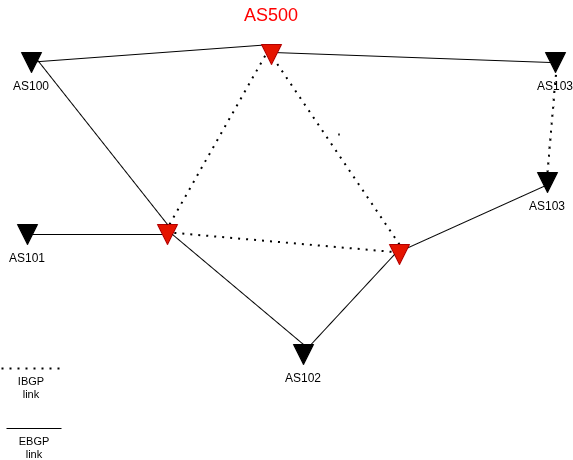
\includegraphics[width=0.7\linewidth]{bgp5.0.drawio.png}
    \caption{simple BGP network, showing both IBGP and EBGP links}
    \label{fig:diag5.0}
\end{figure}
% diagram shows two ASes with internal structure, ASBRs as edge nodes, links labelled as IBGP
% and EBGP.  one AS at least should have 3+ nodes to show the `mesh'
\subsection{Why does IBGP exist?}
IBGP is defined in the base specification for BGP, RFC4271\cite{rfc4271}.
IBGP has two roles in any AS which is part of a multiple-AS system - and it may
also be used for more general network architectures, though more often when BGP
is used as an `internal' network protocol, for example, in data-centre, many,
most or all BGP relations may be EBGP not IBGP, for reasons which will become
apparent shortly.  In this context, however, the topic is purely the usage of
IBGP, and EBGP, in the context of Internet routing (IDR).

One role of IBGP is to carry external routes between border routers in a
transit AS.  The routes exchanged are used both to enable actual forwarding
between ASBRs, and also to inform downstream external networks that those
forwarding paths are available.  Note that it is important to use BGP rather
than some other routing protocol for this role, because it is vital that every
attribute associated with a route is transparently conveyed across the AS,
subject only to specific intended changes to attributes.

\textbf{Figure \ref{fig:diag5.0} shows a simple BGP AS topology with both IBGP and EBGP links.}

Another role of IBGP is to provide some essential subset of external routing
that is required by routers and hosts located within an AS, in order to either
forward transit traffic or enable hosts within the AS to make contact with
external hosts. Unlike the first IBGP role, which must use BGP in order to
preserve exactly route attributes for re-advertisement, the internally
terminated BGP sessions could, in principle, be replaced by some other routing
protocol.  On occasion, and most often inadvisably, network managers may
'import' BGP routes into the IGP.  More often, and less obviously in poor
judgement, IGP routes may be imported into BGP.  However, this rarely makes
sense either, since in general EBGP is used to advertise larger route blocks
than an internal network deals in, so the actual `local' addresses of an AS are
more often written in BGP configuration as static values, for export to
external peers (over  \emph{EBGP}).  So in fact there are multiple overlapping
functional roles for IBGP:
\begin{enumerate}
	\item enable transit traffic forwarding
	\item enable BGP route transit re-advertisement
	\item enable internal host outbound optimal routing (but note that for most uses, internal host connections to external have no need at all of BGP - the IGP simply distributes a `default' route which ensures external ('internet') traffic is carried to the nearest border router.  BGP would only be required if a complex AS had a need to explicitly route externally addressed traffic via specific exit nodes. And, in this case, the larger question might be how to achieve the same effect for traffic in the reverse direction, a problem which IBGP alone cannot solve.)
\end{enumerate}

\textbf{Figure \ref{fig:diag5.1} shows a BGP AS topology with border routers (ASBR), and now also, core routers.
\footnote{There is a deliberate mistake in this diagram!  Not all ASBRs are directly connected - even though a path exists between them all, the unpeered ASBRs will not learn each other's routes.... (Unpeered core routers lead to different but equally catastrophic outcomes.)}}


\begin{figure}[H]
    \centering
    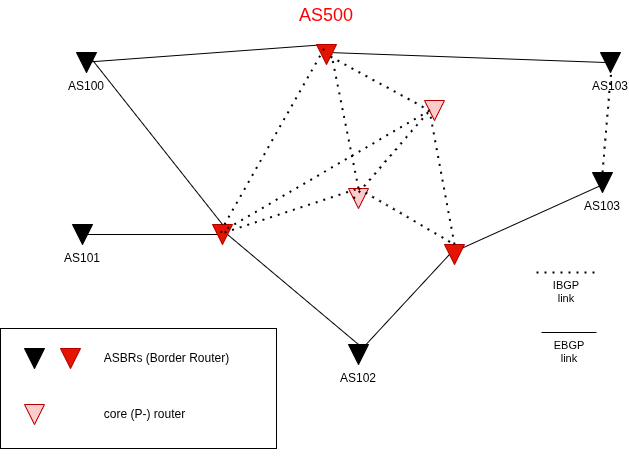
\includegraphics[width=0.7\linewidth]{bgp5.1.drawio.png}
    \caption{BGP network, showing ASBR and p-routers.}
    \label{fig:diag5.1}
\end{figure}

% {\color{blue} insert new diagram (2)}
% diagram shows an AS with ASBRs and P routers, the P routers are smaller.
% there should be a user-plane path through ASBR-P-P-ASBR,
% but only control plane links for all ASBR-P combinations
% Show the P router aggregate as `fabric'.

Note that the distinct functions of ASBR - to - p-router and ASBR - to - ASBR IBGP links enable respectively 1) transit traffic forwarding and 2) BGP route transit re-advertisement.

\subsubsection{Why and how does IBGP differ from EBGP?}
The important point is that, at the `wire level', IBGP and EBGP are almost
entirely identical.
There is just one visible distinction, which is that the route attribute \textbf{Local Preference} is \emph{always} present in IBGP Update messages, while for EBGP
\textbf{Local Preference} is \emph{never} present.
\footnote{Some, but not all, BGP speakers will disconnect a BGP session if this rule is broken.}
All other distinctions, while
absolutely vital, are observable only by observation of how routes received are
re-advertised differently or not re-advertised at all; there are two main IBGP
specific behaviours:
\begin{enumerate}
    \item IBGP re-advertisement does not extend the AS-PATH list attribute
    \item IBGP does not re-advertise routes to other internal peers that it learned from internal peers
\end{enumerate}

%%% {\color{blue} insert new diagram (3)}
%%% this seems a new and hard kind of diagram....
% show the updates at each stage - EBGP -(ASBR) - IBGP - (ASBR) - EBGP
% path attributes that change - LP added, AS path incremented

These two variations are really two sides of the same IBGP
principle/distinction, which is the suppression of the core BGP loop prevention
and path optimisation algorithm.  The consequence is extreme: it means that
IBGP \textit{cannot} independently operate as a routing protocol at all: there is no
mechanism in BGP itself to allow valid paths via internal nodes to be discovered.   Only when
every ASBR directly connected to every other ASBR, is it possible to avoid
having to use some additional IGP protocol to direct transit traffic.
This dependency on a second, IGP, routing protocol is not oversight, rather it
is fundamental to IBGP architecture, such that the IGP metric is explicitly
defined as an input into IBGP route selection.	To complete the explanation:
IBGP announces external routes and as part of the route announcement gives the
'next-hop' address for the egress node, where the next-hop address is known in
the IGP.  Thus, IBGP forwarding works by finding a forwarding path which would
be valid for packets addressed to the associated next hop.	As long as the IGP is
functioning correctly, then every intermediate node forward packets to the
correct ASBR using the following logic:

\begin{enumerate}
	\item first, lookup the internally reachable address (nexthop) associated with the destination external address, in the BGP table which is expected to be consistent across the AS, once the AS IBGP has converged for this route.
	\item use the IGP forwarding table to find the path to the internally reachable address (nexthop) found in step one.
	\item  forward packet using the path from step two.
\end{enumerate}

As long as the internal BGP tables all agree, the packet will follow the IGP
route prescribed toward the egress node's internal interface.
When the egress ASBR is reached, the ASBR uses its BGP derived forwarding table
to choose an external facing interface.  Note, the ASBR BGP route table mirrors
the internal ones except that at the ASBR the next-hop stored in the BGP table
is of the external peer.  The difference is because when the ASBR published the
route to IBGP is substituted the nexthop it received for its own internally
reachable address.  This change of nexthop is another typical aspect of IBGP at
a border node - however, change of next hop is a normal behaviour for BGP under
any circumstance of re-advertisement - it represents an instruction to direct
traffic \emph{through} the BGP router in question, rather than \emph{around	it}.

\subsubsection{fragility of IBGP, and the retirement in most ISPs of internal BGP speakers}

One critical point emerging from this description of IBGP function is the
importance of full BGP level connectivity between all traffic forwarding nodes
within an AS - it is essential that every internal node is (BGP) connected to
all ASBRs, because it is only from direct BGP peer sessions with ASBRs direct
that external routes can be learned.  Even one failed IBGP peer session leads
directly to high probability of lost packets, because the incompletely connected intermediate node
may still be on an IGP best path for some transit traffic - even when it does have a BGP session over
which to discover the nexthop for transit packets - so, any packets addressed to
routes currently served by the un-peered ASBR will not be forwarded correctly,
and therefore will be dropped, at risk otherwise of creating routing loops.

This fragility exists even if all ASBRs are directly connected, however having no intermediate internal nodes reduces the number of peering sessions required, and makes it easier to detect misconfiguration, which otherwise is subject to the vagaries of the IGP as to whether packet loss can occur.
This simplification is (one) goal of the introduction of MPLS in IDR.

However, one improvement in transit network architecture has at least simplified
the operation of transit networks by removing the need for `full-mesh IBGP' -
meaning, the requirement to distribute full route tables to all internal
routers in an AS.  The change is the introduction of MPLS as a transport layer
within an AS.  By converting internal routers to operate as MPLS label switches
rather than plain L3 forwarding systems, the responsibility for delivering
transit packets from ingress ASBR to egress ASBR has been moved from hop-by-hop
L3 address based forwarding, to an end-to-end predetermined path (`source
routed') concept.  In this case, the IGP is generally still used to setup MPLS
paths between ASBRs, with the possibility that specific traffic management may
be applied to optimise certain flows.  The ASBR function remains otherwise
largely unchanged: the main difference being that the forwarding plane logic at
the ingress ASBR, of selecting forwarding treatment based on the nexthop
advertised by the egress node, is enabled to be a MPLS forwarding rule rather
than simple L3 FIB lookup resulting in an egress interface.  Instead, the
egress interface specification includes an MPLS label stack, and that label
stack is assigned based on the IGP constructed MPLS path to the egress ASBR
nexthop.

{\color{blue} insert new diagram (4)}
% reuse the diagram with internal P routesr
% keep the routers, lose the IBGP
% draw in `tunnels' over the Ps

\subsubsection{Route Reflection}
Route Reflection is relevant in this thesis context for two rather distinct
reasons:
\begin{enumerate}
	\item it could contribute a technical aspect to a concrete implementation of PIR
	\item it illuminates some general aspects of attempts to extend BGP
\end{enumerate}

In brief - BGP Route Reflection (RFC4456) is well described by the full title
of the RFC: \textbf{\textit{BGP Route Reflection: An Alternative to Full Mesh Internal BGP
(IBGP)}}.

\paragraph{Route Reflection}
 (BGP-RR) is an extension to IBGP behaviour which allows
specific IBGP speakers to readvertise routes within an AS. BGP-RR adds two new
types of Route Attribute, including a list structure analogous to the external
AS PATH used in EBGP.  BGP-RR defines new rules on readvertisement of routes,
differentiating between regular IBGP clients and peer BGP-RR speakers.  An
important property of the BGP-RR design is that the regular IBGP clients do
not need to understand BGP-RR, and so gradual and non-disruptive transition to
use of BGP-RR is made possible.  The lesson from BGP-RR for a prospective
extension of IBGP is that even rather small change in IBGP principles required
significant changes in both the BGP protocol, and in the rules that govern it,
but was possible in a way which did not require change to the existing deployed
system software (but doe require configuration change, albeit mostly just
simplification).

% {\color{blue} insert new diagram (5)}

\begin{figure}[H]
    \centering 
    \begin{subfigure}{0.48\textwidth}
        \centering
        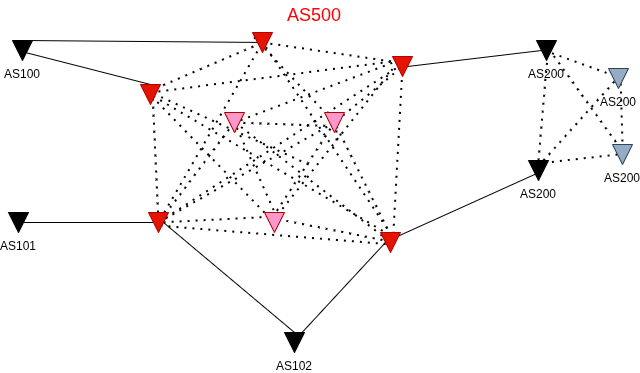
\includegraphics[width=\linewidth]{bgp5.2.a.png} 
        \caption{Before Route Reflection}
        \label{fig:Before Route Reflection}
    \end{subfigure}
    \hfill 
    \begin{subfigure}{0.48\textwidth}
        \centering
        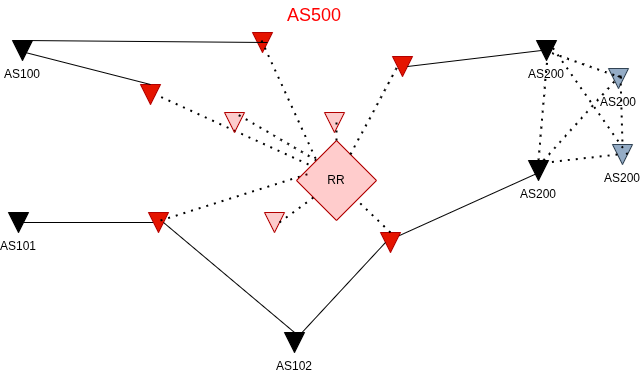
\includegraphics[width=\linewidth]{bgp5.2.png} 
        \caption{With Route Reflection}
        \label{fig:With Route Reflection}
    \end{subfigure}

    \caption{Route Reflection - Before and After}
    \label{fig:Route Reflection}
\end{figure}
% images/bgp5.2.png images/bgp5.2.a.png

% the RR digarm is a bit `stock'
% draw a before and after, with reduced number of links
% note in this fig - `note that RR breaks the no BGP between `P' router rule...

BGP-RR is highly relevant to PIR, if only because it represents the first
generally accepted change to BGP in the direction of centralised control.
However, perhaps a reason that BGP-RR found ready acceptance is that it is very
carefully designed to exclude the concept that a BGP Route Reflector should do
anything more than provide a transparent aggregation function for peering
sessions, in order simply to enable better scalability in a regular BGP AS.

\emph{A good question might be:} how is it that a `centralised controller' such
as a BGP Route Reflector, cannot easily be adapted to become a more directive
and prescriptive actor, rather than a passive tool?  A short answer is that the
crucial role in route selection in standard IBGP is performed only at route
ingress, which is to say, in the calculation of Local Preference.
As RFC4456 says, in Section10:
\begin{myquote}
	10 Implementation Considerations

	Care should be taken to make sure that none of the BGP path
	attributes defined above can be modified through configuration when
	exchanging internal routing information between RRs and Clients and
	Non-Clients.  Their modification could potentially result in routing
	loops.

	In addition, when a RR reflects a route, it SHOULD NOT modify the
	following path attributes: NEXT\_HOP, AS\_PATH, LOCAL\_PREF, and MED.
	Their modification could potentially result in routing loops.

\end{myquote}

And since BGP speakers receiving internal routes are similarly constrained - 
in RFC4271:
\begin{myquote}
	9.1.1.  Phase 1: Calculation of Degree of Preference

	....
	If the route is learned from an internal peer, either the value of
	the LOCAL\_PREF attribute is taken as the degree of preference, or
	the local system computes the degree of preference of the route
	based on pre-configured policy information.	\emph{Note that the latter
	may result in formation of persistent routing loops.}
	....

\end{myquote}

it is clear that the only point in an IBGP or IBGP+RR network for making policy
based evaluations of routes is at the ASBR entry point of a route.

\subsection{Standard IBGP}
In order to reason about modifying the behaviour of an IBGP network, it is
necessary to articulate its standard behaviour, with some focus on the ways in
which the interactions which underpin the collective behaviour of an IBGP mesh
work, and why it may be difficult to adapt the model to support concepts of
centralised or external control.  Here that is done(explained?).

An AS with more than one BGP speaker can be called an `(I)BGP mesh'.  In the
simple version of a BGP mesh, every border router is connected to every other
via BGP (of course, all routers in the AS are connected over actual network
links, and participate in some IGP, such as IS-IS or OSPF).  But critically,
every BGP speaker is \textit{BGP peered} directly with every other BGP speaker.

It should be obvious that every border router must be a BGP speaker, but less
obvious that internal routers should be.  However, in a simple BGP network
every router in the data-path for transit traffic must hold a full routing
table, and since carrying full route tables in other protocols - IGPs - is
known to be impractical, it means that every router must run BGP, otherwise the
internal routers will not have forwarding state for transit traffic.  This is
the classical hop-by-hop forwarding network architecture - modern networks
avoid the problem of having to run BGP on internal routers by tunnelling
traffic with MPLS.
But, for our analysis, we can disregard internal routers, on the assumption
that under either classical or MPLS modes, their forwarding paths can be managed
without impact, since they are controlled directly by the edge (ASBR) routers.

It is important to realise the critical importance of the integrity and completeness of the mesh, in the sense of every router being fully connected to every other, via BGP: just one missing link can lead to catastrophic misrouting.  This may appear to create a large number of potential single points of failure, at every link and interface in the mesh.  But there is an easy solution for this: as long as a functional IGP is in place, then BGP signalling traffic can always reach a mesh member unless it become completely disconnected.  The only requirement is that each BGP router uses an internal `loopback' address, rather than an interface address, for it's BGP sessions.  In this way, signalling of BGP can continue seamlessly under any amount of physical or layer 2 connectivity disruption.  

\subsubsection{IBGP - Core Principles}

The differentiated behaviours between IBGP and EBGP emerge directly from the core BGP specification in RFC4271:
\begin{enumerate}
	\item A BGP speaker identifies an internal (IBGP) peer simply by noting at the time of establishment of the peer session that the two peers share an identical AS number
	      % ( AS numbers are exchanged in the BGP session establishment messages)
	\item The AS path list attribute is not extended on routes sent to IBGP peers
	\item IBGP peers do not readvertise routes received from other IBGP peers
	\item IBGP peers on the AS edge use the route attribute Local Preference to inform their IBGP peers of the calculated `value' of a route
\end{enumerate}

\paragraph{IBGP Convergence}

An IBGP mesh operates on a distributed consensus principle: for every
destination prefix, one or more ASBRs may hold an advertised route from an
external peer - and the only goal of the IBGP mesh is to select just one of the offered
alternates, and ensure that the consensus selection is then adopted by all border
routers, including those that hold competing alternative routes.

The mechanism for reaching consensus and distributing the outcome is simple:
every ASBR receiving an external route directly evaluates the quality of the route, reducing the quality metric to a simple, single, linear value, which it then stores, as a persistent property of the route, in  its local RIB (AdjRIBIn (post-filter)); if at this ASBR there are multiple routes to the same destination prefix then only the best according to the Local Preference metric is eligible to be advertised internally; when a route is advertised \textit{internally}, then the first calculated metric is included as a path attribute named \textit{Local Preference}.

All other routers in the IBGP mesh will receive this advertised route, and possibly also
other routes, from other ASBRs, with alternatives for the same destination prefix(es).
As ASBRs receive routes from their IBGP peers, they do not re-evaluate them again, rather they trust that the received Local Preference is valid, and simply run the `Best Path' selection algorithm, which is weighted to rank Local Preference above all else.

Only if  there is a tiebreak for first place, based on Local Preference alone, do other considerations come into play:  there are some simple rules for deciding tiebreaks, which need not concern us
here.\footnote{It is possible in principle for a router within an AS to have arbitrary configuration rules which could result in a different outcome than were Local Preference to be followed.
	However, this is almost certain to be ineffective at best, and outright dangerous at worst, unless every router in the IBGP mesh has the same arbitrary rule.  But, this would be perverse - if the network operator wants to achieve a different result, then it is always better to do it by configuration at the route source.}

\paragraph{Route Diversity, Route Suppression and Best External}
In this way, the IBGP mesh rapidly settles on a consensus - which is made explicit by ASBRs withdrawing their own candidate routes for which
calculated Local Preference is not as good as the current AS-wide best; if the better route was already  known, then the ASBR should never broadcast the route into the IBGP mesh.
Therefore, many internal route advertisements are suppressed at source.

% Additional, once a best route has been accepted, other ASBRs may withdraw their
% own offers, leaving the current best as the only known route.
This behaviour aligns with `normal' BGP semantics, which dictate that a BGP
router only ever advertises routes which correspond to its own selected best route,
and therefore also the route which it uses for forwarding traffic.

However, this behaviour makes recovery from loss of the current AS-wide best slower,
because as the old best route is withdrawn, all alternates have to be again
advertised and a selection process performed, which might have several transient
states.  A popular optimisation is called `Best External'\cite{marques2012}, under which a BGP
speaker may advertise an external route which it `knows' is not best, and which
it does not itself use for forwarding.	This strategy ensures that when a
network wide best route is removed, the new best route may be more rapidly
selected over the whole network.

It's noteworthy that `Best External' enables a curiously perverse behaviour\footnote{Of announcing a route which it does not itself install in its local FIB} for a BGP speaker with forwarding capabilities, and in doing so illustrates some valuable lessons for would be innovators in BGP architecture:
\begin{itemize}
	\item BGP implementer at least are not averse to breaking-all-of-the-rules, when it suits them, when there is  reasonable confidence that the effect is benign
	\item BGP users are also not averse to using BGP modifications, as long as they believe the consequences are not catastrophic
	\item perhaps one reason that `Best External' has not been strongly opposed is that it is a purely internal (IBGP) tweak
	\item the reason that `Best External' is considered safe is precisely that the actual regulation of IBGP behaviour which makes it safe - i.e. rigid adherence to the IBGP consensus mechanism, which demands strict adherence to all of the IBGP specific procedures and constraints - is rigidly enforced.
	\item in spite of wide stakeholder acceptance, up to the level of implementation and use, in the end IETF was unwilling to endorse it; although a standards track product of IDR WG, it is now no more than an expired draft RFC
\end{itemize}
So, a useful and provably safe extension to IBGP has a strong prospect of adoption and implementation by the active stakeholders, if rather lower prospect of endorsement in IETF.  Key properties for acceptance are probably evident safety, and simplicity.  The fact that it could be turned on incrementally, and off very quickly, is also powerful reassurance for cautious adopters.\footnote{The fact that earlier versions of BGP4\cite{rfc1771} specified this behaviour may also help its case}

\paragraph{AddPath and Route Diversity}

\textbf{Advertisement of Multiple Paths in BGP (RFC7911) ('ADDPATH')} \cite{rfc7911} is at once hugely impactful for BGP implementations, and yet also rather trivial.

The major impact is on the low level encoding of a BGP message - for peer sessions that apply ADDPATH, the wire-format representation of prefixes - `NLRI' -  is transformed in a way incompatible with classical BGP.  In classical BGP IPv4 Prefixes are between 1 and 5 bytes in size, and their actual size is encoded implicitly in the first byte, so no delineation between prefixes in a list is required, in spite of their variable size.

In contrast, under ADDPATH operations, the 1 to 5 byte size of a prefix increases to the range 5 to 9 bytes, because a new `PathID' is attached to each individual prefix.  Even though, in most cases, a block of prefixes with a common path could in principle `share' the same PathId, it's entirely possible that in certain cases the PathId's would diverge, hence the requirement to add the PathID element to every prefix, not just every route  - even though PathID is assigned locally by the BGP peer originating the announcement, and has purely local significance to the peer session on which they are carried.  Thus, an implementation of ADDPATH must implement and selectively enable a variant parser and deparser for NLRI in ADDPATH mode (similar considerations to the IPv4 case also apply to IPv6 and other address families.  There is a practical first impact of this aspect of ADDPATH, which is that the bandwidth requirement for ADDPATH enable BGP signalling traffic can be expected to nearly double, even if only announcing just one route per prefix.

A second major impact of ADDPATH on BGP implementations is that the rules for keeping track of routes in the RIB (AdjRIBIn and LocRib) change, if only subtly.  If the `BestPath' selection process is ignored for the moment, the only change due to ADDPATH is that the extended prefix should be treated as the new key - so two routes with the same prefix, but differing PathId, should be treated as different `prefixes'.  This means for example that the rules for replacement and withdrawal of entries in AdjRIBIn and LocRib are working using the extended forms for the purpose of identity.

However, when it comes to selecting BestPath, then, for a given destination prefix, all routes to a prefix, must be considered. regardless of PathID, including also those with no PathId  at all(recall, ADDPATH is enabled per peer, so there may be a mixture of ADDPATH and non-ADDPATH prefixes in LocRib.)  And, if a chosen path is one received adorned with a PathId, it makes no difference to the way that the subsequent route processing functions than if a plain route is chosen.

When it comes to advertising routes the case is also not so complex - it is \textit{compliant} to simply readvertise only the single route which is overall best, in which case the observable distinction is only that towards peers enable for AddPath encoded transmission, the route would be attached to a prefix with some arbitrary PathId, which need only ever be the same in every case.

A different behaviour arises only if the BGP speaker is configured to send multiple routes, in which case additional routes must be distinguished from the best by use of some other PathID, though it matters not what PathId values are used, as long as all are distinct.

\subparagraph{How is the impact of ADDPATH trivial?}
The answer is that, for a receiver of AddPath diverse routes, AddPath is no more complex to manage  than is BestExternal - the important point is that in spite of their being a wider range of routes in view, the same rule for selecting best is still applicable, and must be aligned between the originators of the routes in IBGP and the receivers.  So, although other routes may be sent, there is no room for ambiguity as to which is valid.  The sole function of sending more than a single route is to allow that if and when the primary is withdrawn - explicitly, by use of the prefix, and it's PathId - then, a secondary route from the same IBGP peer is immediately available as a candidate for the new best route.\footnote{This is not intended as a in depth analysis of the use-cases for Add-Path.  One use is for Route Reflection, to enable RR clients to choose routes based on IGP metric, rather than have the RR attempt to do so.  The other is to pre-populate the best backup path in forwarding hardware, when that alternate route is announced by the same source as the primary (again, most likely a Route Reflector).  The `pre-programmed backup path' explains why simply replacing one route with another is not as effective as first advertising the secondary, before withdrawing the primary.}

\subparagraph{Why is ADDPATH significant in this context?} - because `PIR', the BGP Protection application developed for this project, uses ADDPATH as a solution to gaining visibility to alternate routes that may be `better' than the routes selected by ASBRs as primary routes.

\paragraph{IBGP Loop Prevention}

The principle  \textit{IBGP peers do not readvertise routes received from other IBGP peers}
is not entirely intuitive, and is sometimes described as `loop prevention', which is true but not as simple as the following
% diagram and
explanation illustrate:

% {\color{blue} insert new diagram (6?)}
% obvious diagram, a lot like some of the earlier ones

In standard IBGP (pre-Route Reflector), every ASBR links every other ASBR, and since external routes can only be injected at an ASBR, it's rather obvious that ASBRs would only need to listen to other ASBRs.  Moreover, the only reason that an internal, non-ASBR router (a `P' router) should need a BGP route table at all is in order to forward traffic, based on routes learned from ASBRs.  So clearly, `P' routers can have nothing of interest for an ASBR to learn. \footnote{in principle, there may be some AS internal routes wanted in BGP, but injecting them at a `P' router is in general perverse, since any ASBR will do, and making a `P' router an essential source of important routes would be an unnecessary source of additional failure modes.} Hence the rule \textit{IBGP peers do not readvertise routes received from other IBGP peers} is really a statement that `P' routers are only ever route-receivers, which is perfectly sensible.  The fact that it also prevents route-loops is almost incidental.

\subsubsection{Corollaries, Caveats}
Border routers, and all BGP routers, have high levels of autonomy - for example,
it is possible to write configuration rules that prevent an IBGP from accepting
any particular route, for example, one BR in an IBGP mesh could arbitrarily
`reject' routes from some other specific IBGP peer.  Whether this would be `useful'
is doubtful - but the resulting damage would be purely local to the perverse
router's externally connected clients.

More concerning might be the capability for a border router to `overstate' a
route it
originates in the mesh - a badly configured router could very easily direct most or all
transit traffic to itself, by advertising all viable/known routes with a maximal
Local Preference.
This illustrates the point that, within an AS, a very high degree of trust is
required - the power to evaluate an external route is delegated entirely to the
edge router that first receives the route.
Therefore, in any practical BGP AS network it is usually assumed that every
border router applies the same policy in the evaluation of routes - the Local
Preference calculation.
Anything else would mean that the AS as a whole would behave inconsistently.

Note: applying \textit{the same policy} is not exactly the same as applying \textit{the same
rules} with the same outcome - for example, it would make very good sense to
prefer routes received over peer or customer links to routes received over
transit/provider links.
The same policy on different routers or different peers will produce different, but consistent outcomes.

Summarising,
\begin{myitemize}
	\item Local Preference will always dictate the outcome of all IBGP route selection;
	\item  Local Preference is calculated only once, at the point a route is received
	\item Local Preference calculation must be done in a consistently, based on business priorities, expressed as \textit{policy}, and applied at the point of entry to the network.
\end{myitemize}

Then, as long as the \textit{policy} expression is well-formed and effective, 
the network can operate entirely without central control, and this distribution
of responsibility for route evaluation provides for high levels of scalability
and resilience.

( The main issues for scalability being the degree of interconnection required,
however just as MPLS largely solved the problem of scale fore internal routers,
Route Reflectors solve it for edge routers, without changing the overall
architecture as far as the question of policy application is concerned. )

\subsubsection{Other IBGP Specifics}
IBGP usage has aspects not mentioned above which are essential to pragmatic operation of a Transit AS.  It's a curiosity of BGP that whilst the IETF specifications are in many ways detailed and complete, alone they cannot be used in isolation to understand or describe real world usage which is nonetheless so consistently embedded in operator practice.
Fortunately, other resources exist, which largely fill in the gaps between RFCs, and almost as usefully as filling gaps, act as sign-posts to RFCs, especially `informational RFCs.
Three important resource classes are:
\begin{itemize}
	\item industry forum presentations - especially, `NANOG'\footnote{North American Network Operator Group}
	\item publications of Regional Internet Registries RIRs
	\item leading vendor technical documentation and training material
\end{itemize}

For the purpose of succinctly explaining and validating the `missing' essential elements of IBGP, two NANOG presentations suffice well
\begin{itemize}
	\item BGP Communities: A Guide for Service Provider Networks (NANOG40, 2007) \footnote{https://archive.nanog.org/meetings/nanog40/presentations/BGPcommunities.pdf}
	\item BGP Techniques for Internet Service Providers (NANOG50, 2010)\footnote{https://archive.nanog.org/meetings/nanog50/presentations/Sunday/NANOG50.Talk33.NANOG50-BGP-Techniques.pdf}
\end{itemize}

The two essential `hidden' aspects of (transit network) IBGP are:
\begin{itemize}
	\item BGP policy configuration ('route maps')
	\item BGP communities
\end{itemize}

\paragraph{Side Note: BGP `Complexity'}

It is a frequently heard observation, or even complaint, that `BGP is \textit{so} complex': often it seems with the underlying message that `BGP is \textit{unnecessarily} complex'; and it seems often that the complaint is driven by the sight of the often very large and unstructured configuration files which are required to operate a transit network effectively.  But to the extent that the complaint is driven by the size and structure of configuration, it is surely misplaced: the problem, if there is one at all, lies not with BGP but with use that BGP is put to: no other routing system is even capable of performing the task that BGP performs; and to complain about the complexity of configuration is no more valid than complaining about the computer language in which a compiler is written, simply because the reader cannot understand easily how the compiler works.
The reader/complainer should surely go on a course to learn about compilation techniques, and then be sure to take a few months or more to learn well the implementation language (and perhaps a few other languages as well too), before believing that they are qualified to assess whether a particular compiler is `over complex'.

In the opinion of \underline{this reader} (of BGP configurations), the problem with BGP is not that it is too complex, rather that it is not sufficiently complex - programs written in assembly language are also often `too complex' - as well as entirely unportable - and lack of portability which is also a problem from which BGP configuration policy suffers.

\bigskip

\paragraph{We return now}
to the topic of the core use-cases in IBGP for `route maps' and BGP communities, whereby hopefully some of the aversion to BGP complexity may be dispelled, with the benefit of understanding the motivation.

The background to this section can be found in either the `academic' track, or IETF track:

The academic track starts at Gao and Rexford's seminal work, "Stable Internet Routing Without Global Coordination" \cite{gao2000}(2000), and a second paper by Gao, "On inferring autonomous system relationships in the Internet"\cite{gao2001b}(2001), introduced to the wider world the expression "valley free routing", although the concept is deeply embedded yet never used in the first more theoretical paper.   There follows a great volume of subsequent academic work on the topic.  ( The more recent paper \fullcite{shao2021} is an excellent and up-to-date and rigorous treatment of much what follows here.)

In the IETF track RFCs 7454\cite{rfc7454} and 7908\cite{rfc7908} provide more practical perspectives.  However, Gao and Rexford's paper alone is sufficient to immediately understand and apply the basic principles described here, and their terms can be used directly:

\subparagraph{Problem statement}
A transit ISP  - indeed any Internet connected AS network - can cause instability , service failures and fatal loss of revenue or unwanted costs - if it fails to limit the traffic which it receives.  The mechanism to prevent this class of failure is simple: received routes must be very selectively readvertised - if in doubt, leave it out".  In particular, do not allow networks which are not `customers' to send traffic to destinations which are not themselves `customers'.

There are some parallels with the EBGP/IBGP dichotomy in this, however rather than two classes of entity, there are three:
\begin{myitemize}
	\item customer
	\item peer
	\item provider
\end{myitemize}
and there is no `built-in' rule which allows the rule to be embedded in software, nor is there a `built-in' rule which enables a peer relationship to be inferred.  But the mechanism described here is an analogue of the built-in rules for EBGP/IBGP.
\subparagraph{Valley-free routing: the canonical solution}
(Hereafter, \textit{Valley-free routing} is shortened to VFR.)

Route processing rules for VFR are defined separately for ingress nodes, that is, for ASBRs which receive routes from external BGP neighbours, and for egress nodes, which are also ASBRs, but working as route originators rather than as route receivers.
\footnote{It may seem obvious that an ASBR should apply locally the same readvertisement restrictions on EBGP re-export as its IBGP peer would, but that behaviour is not automatically applied for the mechanism described here.  It's a valid criticism of the low-level basis of implementing policy in BGP.

	% the issue here is an anlogue of the hard corner-case where multiple routes received at a single ASBR upset an otherwise simple mecahnism for optimising route selection
	The problem is this: the selective export rules at an ASBR are triggered by the presence of route attributes (Communities) added at the ingress ASBR.  But, at the ingress ASBR, if route export is based on the communities present in the route as received, then the rules will not be applied.  It's problematic in some BGP implementations, and it is not unknown to find parallel configuration blocks which apply the same logic to local (EBGP) route readvertisement and readvertisement of IBGP routes, in order to achieve the `obvious' intention of a single policy.  Even if the BGP implementation does provide a workaround, it's also possible that a less experienced network engineer may make the mistake of not understanding that such a problem exists.}

The rules are:
\begin{description}
	\item[ingress node] The ingress node role is classification and marking.  The principle is simple: every external peer is statically categorised as exactly one of:
		\begin{itemize}
			\item customer
			\item peer
			\item provider
		\end{itemize}
		The classification of a route is simply the classification of the peer that originated it - based on some static list.

		In the simple case three (mutually exclusive use) communities may be defined, though only two are needed, since the absence of either of the others implies the third.  For example, since customer routes are generally `always' re-advertised, they need not be explicitly marked, as long as the others always are.
	\item[egress node] At the egress, the action taken depends on both the classification of the prospective recipient of a route,and, for each route, the classification of the route originator.  There is a simple decision table:

		\begin{tabular}{ |p{2.5cm}|p{2.5cm}||p{2.5cm}|  }
			\hline
			% \multicolumn{4}{|c|} {}\\
			\hline
			Ingress Class & Egress Class & treatment   \\
			\hline
			Customer      & Customer     & readvertise \\
			Customer      & Peer         & readvertise \\
			Customer      & Provider     & readvertise \\
			\hline
			Peer          & Customer     & readvertise \\
			Peer          & Peer         & drop        \\
			Peer          & Provider     & drop        \\
			\hline
			Provider      & Customer     & readvertise \\
			Provider      & Peer         & drop        \\
			Provider      & Provider     & drop        \\

			\hline
		\end{tabular}

\end{description}

But, there is a `problem' here!  The rules for readvertising seem to be identical between Provider and Peer!  So, the simple table is insufficient - a priority rule is needed.  For example, when advertising to a customer, this table allows that routes from any source are admissible - but the best option is based on the ordering Customer $>$ Peer $>$ Provider.

In reality, there is often more complexity to the policies applied than described here, which is perhaps one reason why it is not useful to consider embedding more rules into fixed function software than the IBGP/EBGP functional split.

Moreover, customer/provider/peer classification is used for more than just the readvertisement at egress policy - for example, it is good practice to police rigorously what routes are even accepted at ingress from a customer, and also to some degree what routes are accepted from a peer.

But however complex, the principles are simple and stable - classify at ingress, apply policy at egress.

The final observation is this:

why is it even needed to use this explicit expression, especially in the matter of prioritisation, when BGP has `shortest-path/distance metric' path selection algorithms built in?
The main answer is that the customer/peer/provider rules are mostly about service and revenue protection - even if the expected outcome of default BGP might most often provide that same outcome, it cannot be trusted to do so.

The reason that default BGP rules cannot be trusted are manifold - two simple ones are:
\begin{enumerate}
	\item connected peers might try and game the system - direct traffic via `our' network, in order not to pay a transit provider
	\item ISPs typically `game' the AS-path length mechanism by selectively extending AS-paths ('prepending'), for what may be legitimate reasons.  But, it means in general that AS-path length alone is not to be relied upon as a guarantor of another ISPs commercial interests.
\end{enumerate}

But, there is also a hidden complexity in the intersection between default IBGP path selection rules, and community enforced constraints - it is this:

At an egress node a path may be ineligible for announcement, due to customer/peer/provider rules - but the AS-wide selected path - converged on as a result of AS wide Local Preference assignments - might not be the only one received in the AS.  So for the egress node in question, there could be a theoretical route available, but it is inaccessible, because there is a mismatch between policy expressed in the community/route-map domain, and policy expressed in the Local Preference domain.

Of course, in a well-formed aggregate AS configuration scheme, care is taken to ensure that this type of inconsistency does not happen - because, if it does, traffic may be black-holed, or at the very least, routed in a highly suboptimal path.

The conclusion is clear - policy expressed as low level rules without a high-level - probably automated - coordination design, are rather fragile, and can easily result in hard-to-diagnose problems

But, in the alternate world of fully automated configuration schema management, fixing problems locally, applying ad hoc fixes to local configuration files, risks both causing other problems, and also fixes being lost, when the configuration automation system refreshes configurations - or, if the configuration automation system allows manual overrides to be retained, risks perpetuating fixes for problems that no longer exist.

\footnote{'Peer' is more naturally used than (adjacent) neighbour, however in the specific VFR context `peer' has a quite distinct meaning, hence the localised use here instead of `neighbour'.)}

\subsection{IBGP - Conclusions}
The foregoing section sets out the context for experiments in using IBGP to solve new problems, or old problems in new ways, or attempts to modify IBGP to solve those problems.

There are examples of approaches which
\begin{itemize}
	\item use BGP protocol and existing BGP unmodified implementations to achieve important results - the Valley-free routing policy, based on BGP communities and route-maps
	\item changes to BGP implementation (but not the protocol) - Best External
	\item changes to BGP protocol - Route Reflectors
\end{itemize}
collectively, these represent the main `solution-space' which will be explored later, in support of the objectives which are described in part in the next section - \textit{BGP+SDN - A Thought Experiment}.
\clearpage

\section{BGP+SDN - A Thought Experiment}

\subsection{Prologue}

A network engineer in an ISP, looking into the routing state of one of their
border routers, sees a route advertised by a connected neighbour AS.  Perhaps
the route is `best' on this ASBR, and perhaps it is best for the entire AS, or
some partition of it.  Or not.	But, the route has caught the attention of the
engineer - perhaps because it is a route which handles some very large
proportion of their customer traffic, or at least, some important route as far
as the ISP customers are concerned, and therefore also of concern for the ISP, and the engineer.
Or maybe, the route being a /4, he wonders if it is not a `mistake'.

What now can the engineer do about this?

\subparagraph{If the route has been selected already as Best Path}
then, traffic may be flowing - and if the ISP has
a rather good network monitoring system - perhaps using(netFlow, sFlow, IPFIX,
(SNMP?)) - or `DPI' - then in principle the engineer could uncover some
'health' metrics for the flow in question - though obviously, port statistics alone
hardly help.  If a very smart network monitoring system, it might even be
possible to estimate round-trip-time, or packet loss ratios.  More useful still
might be to have historical data for the traffic to this route, for comparison
with current - even more useful might be to know, in the recent past, which
routes (paths, neighbours, ports) had been selected for this destination, and
whether there were any correlation between the paths selected and the
performance, as measured by this `very good monitoring system.

This being 2026, the engineer is no longer a human but an AI, and at least some
of the very useful monitoring and historical data is stored in some `data
lake'.
Still, the question is: what can the engineer do about this?

\subparagraph{In the alternate case where the route is\textit{ not selected}} - even though, the neighbour
peer is reliable, and the link is not congested, and, were it selected it might
be rather a good choice.  Sidestepping the obvious point here, i.e.: if it is
such a good choice, why does policy not already prefer it? (There can be good
reasons for this, e.g. path length variations due to variably applied
prepending.)  So, the engineer might decide to do some kind of selective `ping'
or `trace route', using the advertised route, even though the routing state in
his/her network makes it rather difficult - perhaps the ASBR has some special
feature enabling it, or some combination of MPLS and policy routing allows this
kind of experiment.  Since this network is evidently rather smart, perhaps it
can also report back to the engineer which peer connection then delivers the
return packets for this `route test'.  So, now, the engineer can see if this
alternate route is good, perhaps better that the existing route (of course, the
network monitoring system is also able to report on the current performance of
the route which is selected.)
Rather obviously, if the return path differs from the `correct' one, it is a
strong indicator that the route is probably not correct.

So, for this alternate case, though the question is the same as the first case
- armed with very good data about whether
an alternate route should be selected, or deselected, what can the engineer do
about this?

\subsection{SDN to the rescue?}
We might replace the engineer with a computer, saving money, and providing cover 365 days/year, /24hours/day - the computer never makes `trivial' mistakes, and can directly communicate over gRPC, netconf, YANG, http3, or even SNMP?.

Now the solution lies legitimately in the realm of `SDN'.
But still, there is a set of routers running BGP, choosing `optimal' routes in a distributed process.
While the routers may `speak' gRPC, netconf, YANG, it's insufficient for this task.
What is the method by which a router with a `good' route can enforce its peers that this route
should be trusted over the current best?  What is the method by which the
router announcing a questionable route can be directed to stop announcing it to its
peers?
At a protocol level the answer is simple, but only when the router announcing the route is the active party - the router with a better route can simply assert a higher
Local Preference, and similarly the bad route need only be withdrawn, or
advertised with lower preference.
So, the solution perhaps is simple: the novel SDN-BGP-CONTROLLER simply sends a message to the router with the good/bad route,
to request that the `route in question' should be assigned a different (lower,
or higher) Local Preference. IN other words, the router should selectively  outsource its
'tie-breaker' function to a third party.  But is this possible?

\subsection{SDN has limitations, any other options?}
At this stage, we might observe that if only routers were smarter, then this
outsourced Local Preference evaluation would not be needed...
But there is a problem with (building) very smart routers - which is that, they
need to react very quickly, even when 1,000s, or even 10s or 100s of thousands
of routes change.

But, this is good news, if only for SDN evangelists, because it means
that there is surely still a role for SDN...

\subsection{SDN V2.0?}
So now the issue is clearer - although SDN can detect the `problem', and perhaps,
calculate a solution, but, SDN alone cannot implement that solution.

What is needed is some kind of `modified' BGP router - modified only in so much that it
can be `properly controlled' by the `SDN controller'.  This next-gen BGP router
is obviously not `SDN' - it's just a router, designed as it should have been
since the start.  It implements some new control protocol, but nothing `smart'
- think `reverse-BMP'.

\subsection{Perhaps BGP could be the new control protocol?}
Working on the premise that the missing piece of a solution is a protocol
to modify specific `BGP routes' located in some internal state of a BGP
router; or, more specifically, to change the outcome of the Local Preference
calculation in that router (and also noting that in future, it might be useful
to be able to modify other re-advertised route attributes than just Local Preference)...

If the solution requires a (new) protocol, then obviously,
even if the protocol is not `BGP', still, the currency of
the protocol is in large part BGP encoded route attributes.
The question now is:  are we designing just a protocol,
or a larger `architecture'
- and clearly, if required, the architecture should come first.

Put another way:, if the idea is simply to substitute a post-filter AdjRIBIn route for
another similar route, then whether the protocol is bgp or not is not the
issue, rather, how should the controller frame the context of the request for a
new route, and, how should the controlled router behave?
Important questions relate to how the controlled router should respond as
relevant local and peer router state changes.

One - simple - solution would be simple substitution - the pushed route would
simply replace/override the original (post-filter) route in AdjRIBIn, which is
pushed into tiebreak.

\subsection{Framing solutions based on route substitution directives}

It is easy to propose, at a high-level, a route substitution, which simply replaces the target routers route processing and filter logic at the level of a single route,
but the challenge is how to
define the relationship between an entry in the target router's `pre-filter AdjRIBIn' table, and a substitute outcome of filter application, and how to define the currency and
applicability of the substitution instruction.	There are some extreme cases:

either:
\begin{enumerate}
	\item  match on the precise route, i.e the entire set of route attributes (could be prefix specific, or not).
	\item  match on some `regex' over the route attributes
\end{enumerate}

and also either:
\begin{enumerate}
	\item  retain the override only as long as the specific matched route is in AdjRIBIn
	\item  retain the override indefinitely
\end{enumerate}

Another dimension: route source - the instruction is initially driven by a
route in a specific peer AdjRIBIn.  But. the instruction could reasonably be
intended as to apply to only the specific source, or to any source.

\subsection{A policy defined solution}

It's emerging how to solve this /define this:
The goal is to define a substitution rule, and so far the substituted value is
clear and concrete - mostly the important factor is the assignment of
Local Preference.  The `match rule' is less clear, but only in terms of scope.
This is open to the controller, but too specific a rule may become invalidated by a
trivial change.  The open question is how to define rules which are less
specific.  But, this can be left out of the protocol.  A controller could
choose to issue overrides which are entirely specific. Ambiguous or flexible
matches are also easily defined.
The ability to define `smart rules' would allow for transfer of `intelligence from controller to router.
A router could declare its level of smartness.

\subsection{SDN approach, summary}

The SDN approach requires some form of extended BGP protocol, which allows controlled routers to correlate their existing internal routing table state with override directives.  The reason is that when the controlled router state changes, the target router cannot afford to wait for the controller's next instruction.  We are not \textit{transferring} the core role of evaluating all routes to the controller, just asking the controller to be a source of `hints'.

It's an uncomfortable role for an SDN controller (and there are more challenges still to come...)
\bigskip
But, this is, as titled, only a \textit{thought experiment}.

\section{Implementing external control in IBGP}
\subsection{Implications for exerting control in a distributed IBGP mesh}
We could state the objective in terms of observable behaviour: which is that,
every Border Router evaluates routes based on some enhanced procedure, which
may be informed by external factors, historical data, deep analysis of offered
routes, ongoing network monitoring or probes.
A central part of the sentence is `every Border Router evaluates ...' - i.e. we
avoid the question of how an external agent can exert control by stating that
the responsibility for making `better' decisions is left where it currently
lies - at the edge router which receives a new route.
But, we only are describing the wanted observable behaviour.  And the reason to
do this is to duck the question of how another entity can insert itself into
the
IBGP mesh with the eventual desired effect, as if the border router itself
applied better policy.
\subsubsection{The Importance of (Being) Local Preference}
In classical IBGP networks, consensus is critical.  If ASBRs do not have common
routing state, then the network fails - a packet arriving at an exit node which
does not know that it \textit{is} the exit node will loop or be dropped.  An AS may be
partitioned by IGP based route metrics, but within a partition consistency is
essential.
In this classical architecture, convergence based on Local Preference is the
only mode of operation.
But, an alternate mode can be considered, in which the exit
node once selected at ingress cannot be overridden at the exit - this requires
a tunnelling architecture, which would allow an ingress node to deliver traffic
directly to a chosen egress point, with a defined treatment.
In such a network, convergence on a consensus route is not important.
More importantly, in such a network local preference is no longer central - an
edge node could reevaluate a route and arrive at a different result -
consistency does not matter, the value of local preference is in reducing the
load on other routers.	But, in order for this licence to be useful, other
routes must be exposed.  `Best External' is a good start.
But, this architecture has much more to offer than just Best External driven
reevaluation - once all exit nodes are selectable, another BGP entity can
advertise routes which target those egress nodes, safe in the knowledge that
the alternate paths are viable.

\subsubsection{Design Space}
to make an IBGP mesh behave differently, we might
\begin{enumerate}
	\item  make ASBRs smarter
	\item  work with BGP in some way to allow ASBRs to still be dumb, but somehow overall enable the AS to behave better, whilst still being a traditional IBGP system - which must mean some via some additional BGP speaker(s) with special properties.
	\item  change the architecture
\end{enumerate}

The thesis scope is not to replace BGP, either as IDR or as AS internal
protocol.
And options 1) and 2) are not so different - the distinction is as to whether a
controller can be made effective when limited to using only existing BGP
principles, or instead, define some more powerful scheme which can in effect
make ASBRs smarter, or at least, more tractable.

\subsection{Detailed Analysis Of Conflicts and Resolutions Between Classical IBGP and BGP Controllers}
This section is rather dense in its logic, and essays a rigorous exposition
which justifies the following statements:

\begin{myitemize}
	\item A BGP Controller can be formally defined in an analogous way to a BGP Remote Reflector, with capabilities which are a super-set of a BGP Route Reflector
	\item Neither IBGP nor IBGP + Route Reflection are expressive enough or compatible with a BGP Controller
	\item IBGP + BGP ADDPATH (RFC7911)\cite{rfc7911} provide more relevant expressivity, though still insufficient
	\item IBGP + BGP/MPLS VPN (RFC4364)\cite{rfc4364} provides complementary expressivity to IBGP + BGP ADDPATH, but is also insufficient, alone
	\item IBGP + BGP ADDPATH + BGP/MPLS VPN in combination are sufficient for BGP controller - but, no vendor is known to enable the combination in an viable way.
\end{myitemize}

\subsubsection{Definition of a BGP Controller}
A BGP controller is a system which exerts \emph{dynamic} control over the
routes advertised and implemented within an AS.  It does this by interacting
with ASBRs using BGP and current BGP extensions, or by other means.

\paragraph{Scope of a BGP Controller behaviour}

\begin{itemize}
	\item A BGP Controller cannot `invent' routes.

	\item An AS acting under influence of a BGP controller should not be distinguishable by its behaviour from an uncontrolled AS, other than by inference by observing better or dynamic policy (an example of dynamic policy would be that a route initially rejected or selected may later change status, without any corresponding external route state change).

	\item A BGP Controller may have levels of capability:
	      \begin{itemize}
		      \item The lowest level is purely reactive to specific received routes: when a EBGP peer route is received, changed, or withdrawn, the controlled network selects and advertises a route other than that which ASBR policy dictates. When a later change removes or updates the route which triggered a controller response, the controller must again react in order to exert control, otherwise the override associated with the route is removed.

		      \item  Higher level capabilities

		            \begin{itemize}
			            \item  a more capable BGP Controller may issue directives which are generic or persistent: this would have the effect of protecting the AS from trivial changes to a `bad' route, which otherwise would undo the protective instruction.
			            \item  Orthogonally, a more capable BGP Controller may issue directives which have explicit time limits, or may issue prophylactic directives to ASBRs other than the ASBR which received the trigger route.
		            \end{itemize}
	      \end{itemize}
\end{itemize}

\subsubsection{Policy Versus Configuration versus Dynamic Control}
Conventionally, when an ASBR, and/or an entire AS, receives a `route', it runs
'best path', and either switches to some new route, normally the route received
(but, see MED), or more often, makes no change.  Then, nothing more happens,
until again received external route state changes, at which point the selected
and advertised routes may also change, subject still to Best Path, which is the
concrete expression of the AS policy.
If a BGP controller is introduced then conceptually it interferes with `Best
Path', and therefore, when again a related route change occurs, it must again
directly oversee the response.	IN this scenario, a base \textit{policy} is
implemented as conventional static configuration is each ASBR, and the BGP
Controller in some manner interferes with the AS route selection, but ASBRs
policy is unchanged.  In this case we can understand that the ASBR control
mechanism is a `control plane' rather than `management plane' strategy.
Its important to state that the `smarter' control mechanism crosses a boundary
into configuration ('management plane') - because the ASBR is being give a
'rule' to apply, rather than simply a routing protocol item which affects the
intended behaviour, but which is not identifiable as anything other than
'another' route.  This distinction is central: there might be constructed some
hierarchy of persistence, but still the persistent management plane strategy is
qualitatively distinct for a routing protocol extension.

BGP controllers thus fall into three basic categories:
\begin{enumerate}
	\item The BGP controller uses only BGP and current BGP extensions
	\item The BGP controller uses BGP with customised BGP extensions
	\item The BGP controller uses methods other than BGP, possibly in conjunction with standardised BGP.
\end{enumerate}

Note: The expression `uses only BGP and current BGP extensions' is ambiguous:
one might propose a mechanism which is technically BGP, but not supported by
any known implementation of BGP, and might require behaviour which contradicts
'mandatory' rules for BGP.  For example, the `wire' messages might be entirely
valid BGP, but the aggregate usage undefined.  Therefore, there is a
sub-category, or sub-categories:

The BGP controller uses only BGP and current BGP extensions:
\begin{enumerate}
	\item  in ways consistent with specification and live implementations, such that the actual behaviour corresponds to the intent
	\item  in ways consistent with specification, but with no known implementation, or implementation behaving in the manner intended
	\item  in ways which contradict specification, or reasonable interpretations thereof, and have no known functional implementations.
\end{enumerate}

Orthogonal to these categories of compliance are categories which relate to
mode of operation:
\begin{enumerate}
	\item The BGP controller operates by promoting a received route in order to suppress another route which would otherwise be selected and advertised.
	\item The BGP controller operates by interacting only and directly with the ASBR which receives a route, in order to suppress that route.
\end{enumerate}

\section{Implementation Strategies}

In the hypothetical thought experiment, however complex the rationale for
overriding the default policy outcomes of route selection, the range of
pragmatic options remains very limited:
it is already accepted that at the AS level the main scope for changing AS
behaviour is limited to making a different selection from offered alternatives,
with variants such as specific modifications to routes readvertised, and
potential to advertise distinct routes, or distinctly modified route attributes
at a more granular level.

How then can a controller use existing BGP to achieve a desired outcome of
removing a particular route from selection, or, a more specific version of the
same thing, enforce that another specific received peer route is preferred and
re-advertised?

The question can be deconstructed into two aspects:

\begin{enumerate}
	\item the element of learning of both the unwanted and alternate route, to include also monitoring that both routes, and any potential later arriving better route, remain in view of the control agent
	\item instructing the ASBRs within the AS to promote the alternative route
\end{enumerate}

Note: there can be interaction between action and observation: for example, if
the mechanism for changing the advertised route results in information about
either the deprecated or alternate route becoming stale, then the solution is
incomplete, because there is then no mechanism to react when for example either
the alternate route, or the unwanted route, is removed.

Assuming for the moment that a reliable route monitoring system exists - then,
since the only control plane action available to any BGP speaker which can
impact routes advertised by another is itself to advertise a similar route
which might be chosen instead - the question reduces to what route, advertised
to what IBGP peers, can have the desired outcome?  Clearly, a copy of another
route to the same prefix can be advertised by an IBGP speaker, to some or all
other IBGP peers.  Such a route can be crafted such that it is guaranteed to be
treated as preferred, simply by using Local Preference, or, with equivalent
effect, some additional attribute, e.g. a specific community attribute, for
which the IBGP peers are consistently configure to process with high priority.
However, using Local Preference is preferred because the advertised value can
be adjusted finely so that some  foreseeable and desirable external route
changes may automatically override the override.

So, which IBGP peers should receive this `special' route? It would be desirable
if a minimal distribution list could be effective - it might seem that the only
way to effect the redirection would to send the new route to every ASBR - but,
depending on some AS specific configuration, it may be sufficient to send this
'fake' route to just the ASBR which received the `bad' route from an external
peer, because if doing so forces that ASBR to withdraw the unwanted route  from
advertisement to internal peers, then all remaining peers will simply fall back
to the next `best' route. If the objective is just that - use the second best
route - rather than some other than second best - then, this strategy works,
with just one caveat:
the second best route must not lie also with one of the peers of the same ASBR
as the bad route.

However, the corner case of preferred route and default best route ingressing
at the same peer needs more careful treatment.
There may be a simple twist
which can resolve this: which is to use \emph{EBGP|} as the control channel to
'boost' the alternate route.
This certainly overcomes the problem of how to
force an alternate route selection between two routes received at the same
ASBR.
But, it introduces, or highlights, a different problem, which is one concerning the monitoring channel for the controller.
If the monitoring channel is one such as `Best External', or ADDPATH, then these both
require IBGP peer connections, and have the unstated (and essential) merit, of
conveying not only the existence of alternate routes, but also the calculated
local preferences for them.
The Local Preference of every candidate route is needed in order to calculate
which alternate should be chosen, and with what enhanced Local Preference to
announce it.  Switching to EBGP alone would remove the knowledge about
calculated Local Preference.  But, even if every ASBR is `wired' to the
controller both for IBGP as a monitor channel, and EBGP as a control channel,
still, by installing an override alternate at an ASBR, the Local Preference may
become unavailable over IBGP, because the presence of the new route causes the
monitored routes to be removed in IBGP.  This is even more a problem than it
may seem: if the bad route disappears, then the controller ought to remove the
override, and then the bad route will simply reemerge in IBGP.

Note: in general, this pathological behaviour only arises in the case of an alternate route received at
the same ASBR as the bad default choice.
Note also: if IBGP is to be used as the monitor channel, then certainly either `Best External', or ADDPATH, must be configured - otherwise, the existence of any alternates cannot be discovered at all by the controller.
\subsection{Uses of ADDPATH, NextHop Peculiarities}
We have  observed that for many situations, sufficient route diversity is enabled if BestExternal is activated, to allow a IBGP located controller to receive alternate routes which can be used as a basis for preparing a viable alternative to draw traffic from a path which the controller has determined to be `bad'.

ADDPATH has ambiguous definition and implementations, likely driven by ambiguity of the intended use.  The primary objective of ADDPATH appears to be to aid route recovery when a previously preferred route is withdrawn.  Other use cases \footnote{see for example Cisco IOS XE IP Routing Configuration Guide - Chapter: BGP Additional Paths} include enabling of BGP multipath.  It is implied that the natural `home' for ADDPATH is the RouteReflector rather than an ASBR.   The main point about ADDPATH is that even if overlapping paths are advertised by a single router, unless the paths have distinct next-hops, then the only usable path is the one in the set having highest Local Preference. Some implementations, will only advertise more than one route via ADDPATH when the additional routes would have different next-hops; if the router in question configures `next-hop-self' for IBGP, then this clearly implies that multiple routes will not be advertised.

There is a configuration `tweak' which can render ADDPATH much more powerful, and has the potential to lift ADDPATH into a level of capability which can be very useful for the controller application envisaged here.  The tweak is to disable IBGP next-hop-self while enabling ADDPATH.  In general, in order to have a functioning IBGP forwarding plane, the next-hops advertised should be redistributed in the IBGP IGP, otherwise when an ASBR attempts to install the resulting route in its local FIB it may fail, or worse, install a route which does not resolve to the correct ASBR.

However, this problem can be avoided by only selectively enabling both ADDPATH and simultaneously disabling `next hop self' for BGP peer sessions to a controller.

The combined effect of this configuration strategy is, or should be, that, for normal IBGP sessions, i.e., to all other ASBRs, the `normal' IBGP behaviour is shown - next-hop is always an IBGP mesh internal address, and only the single best route is announced.  Meanwhile, the controller role BGP speaker receives multiple routes whenever they are available .

The last, and required, beneficial aspect of this external next-hop pass-through strategy is that it also enables the controller to issue an effective override route to this ASBR.  Without the external next-hop information, there would be no way for the controller to correctly override the target ASBRs locally preferred route.  But, armed with the correct external next-hop, the controller can  issue a route override which has the desired effect.

There is only one possible catch, which is this - depending on the ASBR router implementation, if it applies the policy of refusing to advertise more than one ADDPATH route per next-hop, then the effect of the override route installation will be the loss of the underlying route from the ADDPATH set, to be replaced by the new `copy' route - which if it happens, invalidates the entire scheme.
However, and at this point we are deep into vendor specifics - but, depending on the implementation, it may be possible  - the case can be rescued by writing an export filter for the (ADDPATH) controller peer session, which excludes the new `fake' route from the ADDPATH list, and thus re-enables announcement of the base route.

There are undoubtedly a large number of implementation dependencies in this strategy - but, were the strategy to be accepted as a `valid' use case, it is plausible at least that even non-conforming vendor implementations could be fixed, so that the scheme could be made functional
\subsection{BMP: An Alternate strategy for route monitoring}

In the previous section the use of IBGP as a control and monitoring channel
were explained: in many cases, a controller can successfully operate by
monitoring routes received over IBGP, and, when action is required, promoting an override alternate route, simply by readvertising an existing route from another ASBR peer, but with higher priority than that set by the source ASBR.
We saw that in the challenging corner case, where the preferred alternate is reached via the same ASBR as the unwanted route, then it may be difficult to exert override control, and even more difficult to reliably
monitor the relevant routes.

It is not clear that a widely applicable solution to this problem exists, with just these tools of regular IBGP.
However, there now exists an alternate scheme for reliably getting route information from a
BGP speaker: RFC7854 - BGP Monitoring Protocol (BMP).

BMP has evolved significantly during the period of this work.
The initial BMP RFC, RFC7854 \cite{Fernando2016}, published in 2016, provided only for monitoring of the `Adj-RIB-In' routing table in a BGP speaker.
In 2019 RFC8671 \cite{rfc8671} introduced support in BMP for reading Adj-RIB-Out, and in 2022 RFC 9069\cite{rfc9069} introduced BMP support for Loc-RIB.
These extensions are, or could be, significant for implementing a BGP controller,
not least because the `Adj-RIB-In' of RFC7854 is not guaranteed to provide calculated Local Preference.
Without Local Preference, a BGP controller is unable to assess route fitness, except by attempting to replicate
the calculation done by each ASBR, and the possibility that the calculation
result may not agree introduces great uncertainty as to effectiveness of a
controller, not to mention a very large additional implementation effort which
amounts to re-engineering the BGP policy language of every potential ASBR in
use.

Anecdotally, different early implementations of RFC7854 BMP varied as to whether
Local Preference was supported or not.\footnote{RFC7854 makes no mention of whether the Ad-RIB-In monitored is pre- or post-filter, nor does the expression Local Preference occur anywhere in the text.}
A BMP implementation does form part of this thesis, however at the time of work no available `software' BGP speaker supported BMP - the implementation was tested with a physical router (Juniper),
but neither the Juniper nor the Cisco virtual routers available for study supported BMP,
nor did any other open source router.
The tested BMP implementation on a physical router was able to provide Local Preference.

For this reason, the analysis of a BMP based approach here is purely
theoretical.

\subsubsection{Using BMP to Implement a BGP Controller}
In principle, a controller could use only BMP to monitor routes, however, doing
so requires that the AS wide route selection be inferred, whereas monitoring
the actual converged RIB by passive participation in the IBGP mesh is
considered to be a safer and simpler approach - it allows attention to be
focused on routes which are an actual threat, because selected, and also to
monitor the effectiveness of an intervention.  It means that the BMP role is

\begin{enumerate}
	\item to select alternate routes, when it is determined that they are required
	\item to reliably monitor the targeted and selected alternate routes for change
\end{enumerate}

Concurrently, IBGP is used
\begin{enumerate}
	\item as the control channel
	\item as the primary threat monitor channel
\end{enumerate}

\subsubsection{Can BMP help solve the same ASBR alternate corner case?}

In part, the answer to the questions of the section title is : yes.  It does so
by enabling reliable monitoring of both unwanted and alternate routes.
However, BMP is purely passive - it leaves open the issue of route override.
However, the part solution of using EBGP can now be fully utilised, since BMP
ensures reliable and continuous route visibility.

\subsection{Controller strategies - A conclusion?}
We have seen that basic IBGP can enable useful degrees of AS programmability,
using just Best External as the route monitoring channel, and IBGP based
directed readvertisement of alternate routes to suppress unfavourable routes.

Additionally, BGP Monitoring Protocol (BMP) can provide an additional solution
for an important corner-case which IBGP alone cannot address, but only by using
complex combinations of BMP, IBGP and EBGP, and also only with certain more
recent/advances BGP/BMP implementations.

However, the full scope of ambition includes other features:

\begin{enumerate}
	\item  dynamic change
	\item  granular control
\end{enumerate}

Moreover, another topic has yet to be addressed, or even explicitly raised, which is preventative control...

\subsection{More Granular Control, via MPLS}

Already mentioned in this chapter is the BGP feature "Advertisement of Multiple Paths in BGP" (RFC7911\cite{rfc7911} -  July 2016).

In conjunction with the RFC "Using BGP to Bind MPLS Labels to Address Prefixes" (RFC8277\cite{rfc8277} - October 2017), a radically different and more flexible IBGP forwarding system can be constructed., one which in the limit approaches the extreme fragmentation level described in the early theoretical section XXX?

The basic concept is as follows: following the concepts of BGP ADDPATH (RFC7911), an ASBR can advertise multiple routes concurrently, of which one is the generally preferred `best path' choice, having the highest Local Preference value at that ASBR. BGP ADDPATH capability enables more than one route to the same prefix may be advertised, and a new attribute (Path Identifier) is introduced to distinguish updates for different routes.
In isolation, ADDPATH is not easily motivated - it does not provide any explicit way in which an internal peer could directly utilise routes which are not `best', nor even `best' routes, in the event that the IBGP mesh has selected another egress router than the ASBR advertising a route with ADDPATH attributes.  Even the question of whether this is an EBGP or IBGP targeted capability is left unresolved in the RFC\footnote{A clue may be found in the original draft title for the RFC, which was "Best Practices for Advertisement of Multiple Paths in IBGP", and a related contemporaneous IETF draft: "Fast Connectivity Restoration Using BGP Add-path"}

RFC8277 explicitly describes use of MPLS next-hops with ADDPATH (see e.g. Section 2.2:
\begin{myquote}
	If the procedures of [RFC7911] are being used, a four-octet "path
	identifier" (as defined in Section 3 of [RFC7911]) is part of the
	NLRI and precedes the Length field.
\end{myquote}

This enables a direct forwarding path to be established, which guarantees that traffic directed into an MPLS tunnel at an ingress ASBR will be directed to the route source corresponding to the advertised path at the ASBR that advertised it using ADDPATH.  Without this capability,  traffic for the selected destination can never be forwarded other than via the AS wide route established by consensus between ASBRs.

Once the feasibility of the principle is established, the remaining task is to implement the feature in a way compatible with the objective of PIR / BGP control: however, the BGP aspect is rather simple: the BGP speaker which implements a controller function should negotiate the appropriate BGP capabilities which permit ADDPATH and MPLS next hops, and the ASBRs should be configured to send two or more paths per received route, where alternatives are received, to the controller role IBGP peer.  Now, the controller can always select an alternate route for the entire AS, by readvertising the MPLS route with uplifted local preference.  Of course, this still requires that all ASBRs support the explicit MPLS forwarding path, even if not ADDPATH.
Variations on the design can reduce the requirement for RFC8277 support by designating an internal MPLS forwarding point which installs a forwarding rule: for example, a BGP controller could integrate the MPLS forwarding plane logic required, on a `P' router adjacent to ASBRs.

There remains a very remote corner-case, which is the possibility that a large number of `bad' routes exist at a single ASBR, such that ADDPATH cannot reasonably be configured to propagate sufficient depth of alternatives than a hypothetical best path at the same ASBR can be obtained.  But it seems doubtful that this represents a serious obstacle to deploying a protection scheme using ADDPATH and MPLS - the more realistic concern is whether the additional complexity required to save the base corner case could be justified.  A simple deployment based on basic IBGP and BestExternal, or including BMP, seems a sensible first step for any deployment of PIR in a protective role.

However, if the use-case is the more general one of `More Granular Control', then ADDPATH+MPLS\_NEXTHOP are well-placed to make this a reality - the challenge then moves into the issue of how to create a coherent management system for a much more complex flow structure, and how to build a service concept which  can take advantage of this revolutionary capability.

\subsection{Dynamic Control, via vanilla BGP}
Even RFC4271 BGP provides that Local Preference may be reevaluated: see RFC4271, section 9.1.2:
\begin{myquote}
	If either the immediate next-hop \emph{or the IGP cost to the NEXT\_HOP (where the NEXT\_HOP is resolved through an IGP route) changes}, Phase 2 Route Selection MUST be performed again.
\end{myquote}

So, the IBGP based controller is at liberty to change its mind, or take its time making up its mind, or even try out an option, and revert if it does not work out - all the while behaving no differently to how a conventional BGP implementation might do.

The obstacle to dynamism is not in the protocol, or the architecture, but purely in the legacy policy implementations, which have no stateful model.  Of course, even the controller should take care to be able to remove a route rather quickly, when the route itself is withdrawn or changes at the ingress ASBR.

\subsection{Policy, Configuration or Protocol?}

The focus in this chapter so far has been on a protocol based strategy to adapt or extend the current IBGP architecture to enable novel behaviours, whilst protecting the essential elements of stability, scalability and performance which epitomise the existing architecture.

However, it may be that an adaptive, yet existing protocol based, approach is not the only possible solution, let alone the best.  In this section, other approaches are considered.  One alternate idea is to use configuration, or \textit{policy}, rather than signalling, to achieve the same high level goals; another is to extend the core protocol, or to graft on to it additional side channel protocols, analogous to other extensions.

\subsubsection{Terminology - `configuration' or `policy'?}
The terms \textit{configuration} and \textit{policy} overlap in some degree: if the term \textit{configuration} were to be used, objections might be that the term is inappropriate, or impossible to implement as device specific configuration, or simply that it causes confusion, while \textit{policy} could be seen as too abstract and ambiguous, and arguably is only a term for an abstract construct, which is eventually always embodied in some form of configuration.

For the purpose of this section, the term \textit{policy} is preferred -  but, it is understood to mean a concrete unambiguous set of `statements', which could, and probably should, be expressed in some DSL\footnote{Domain Specific Language}, which in some cases might simply be the native configuration language of the BGP speaker in question.

In other words, policy is independent of style of expression, and its domain is purely semantic rather than syntactic - and while a formal syntactic form might be desirable, formulation of policy need not wait on formulation of a perfect language in which to express it.

\medskip

As important as the question of policy encoding is the topic of policy dynamics and persistence, for example, if some policy directive is imposed, what then is its scope, in terms of lifetime?

But, if we allow that the policy language \textit{includes} a time related dimension, then the question of persistence can be moved into the policy ontology domain, just as we should expect that a policy directive can also include scope variations, for example `for all peers', or, `for all external peers'; so `until further notice', or, `until next system restart', or `until peer XXX BGP session restart' should be valid qualifiers on any policy directive.

\subsubsection{Explicit Control contrasted with Policy - An Example}
Suppose that a controller determines that some route -  a set of NLRIs with a common path attribute set - is to be deprecated, or entirely excluded from use and external re-advertisement - then, a `policy enabled' controller should send some directive consisting of some `match' term and some `action term'.

The action term is more easily conjectured - e.g.: `set Local Preference 10', or `filter from Adj-RIB-In'.

The match term could vary: it might simply identify prefix and the source external peer, or source adjacent AS: it might match the exactly advertised route prefix, or some subset, possibly as an LPM\footnote{Longest Prefix Match - i.e. where X.X.0.0/16 might be used to exclude several more specific prefixes, even if the actual prefix is not present.} match term.

At it's most specific, a match term might be written as some regular expression over the set of path attributes, or by reference to an ADDPATH Path Identifier.
\medskip

Immediately, it appears that \textit{policy} based control may in many ways be more flexible - and perhaps more useful(!?) - than any routing protocol based system.  That distinction can be made explicit by pointing out exactly the range of policy directives which can be `encoded' simply by using the route-override schema proposed in previous sections: which is to say, the low level action is simply to install a static route which may have higher Local Preference than another, and the time based dimension is `until further loss of peer session with controller'.

If the controller's continuing control is assumed then the semantics may be more specific, but difficult to define in some unambiguous language, unless the scope is limited to the single transaction of install route, then later withdraw it, if replacement itself changes,  or in any case, when the adverse route is withdrawn.  But even this cannot be expressed as policy, because at the policy target the replacement route may not be visible.

In conclusion, although a policy based route override may be superficially appealing, it doesn't seem possible to articulate even the simplest wanted control plane function directly as a (management plane) policy function.  The reason for this is not hard to find: only if the logic which governs the controller can be encoded in a policy directive, can a policy based system provide an equivalent capability to a controller based system.  Moreover, even if the policy language can define a rule which allows the target to behave exactly as a controller would require, it still would require that the target have also the same state visibility as a controller, to the extent that the policy relies on external state.  And, if the policy based expression was a useful long term `configuration', then a better strategy would be simply to use a controller to write policy based static configuration, and rely on an optimised, static, policy management strategy.  Arguably, that position simply represents the current, inadequate, state-of-the-art in IDR management.

\bigskip
In plain language, in answer to the question  "can route attacks be effectively mitigated simply by updating ASBR configurations faster, and with more granular structure?", the answer is a simple "no".
For example, the controller may use an ML analysis to identify a threat, but the analysis may not yield a simple policy rule other than an exact match for every attribute of the rejected path; or, the threat assessment may be based on an external metric - e.g. packet loss, or unexpected traceroute behaviour.  These \textit{cannot} be reduced to a policy language.  The best that could be hoped for is that the controller might, in some cases, be able to write some less specific policy rule which could avoid the ping-pong of threat route being trivially readvertised, then requiring to have the  rule rewritten,  By the controller; but this is at best an optimisation which is clearly not applicable in many cases, and offers no functional advantage.  A better way would be to use `smart' configuration to write those rules which might have long running applicability, and save the controller to handle the cases not addressable by configuration/policy.

\subsubsection{Control using Explicit Addpath Path Identifiers}
At the opposite end of the spectrum to \textit{policy} based control is the idea of extending ADDPATH to support control: when an ASBR advertises routes with ADDPATH, then each specific route gains some form of unique identity - such that it is conceivable that some protocol extension could use an ADDPATH route identifier to launch some further protocol interaction.

This concept appeals, because it potentially solves in a direct way the core challenge - to reject, or demote, a specific route - which can otherwise only be achieved indirectly, and rather inelegantly, by strategy that simply selects and advertises differently an existing route, which is clearly a `kludge' or workaround, rather than a natural extension of the existing architecture.

It is not possible/intended/practical to devote so much attention to this topic (Control via Addpath), although in principle it might be a very fruitful direction for future work, but a few further comments are still useful in the context of this Thesis/work:
earlier, the problem of improving resilience to routing attacks was divided into the separate problems of monitoring route state, mitigating threats, and managing mitigation as routing state changes.
In that context, ADDPATH is seen as a purely passive potential monitoring solution, ranked more widely effective than `Best External', and alongside, if not directly comparable with, BMP.

ADDPATH has no obvious advantages as a pure monitoring tool than BMP, and some disadvantages, i.e. not always can ADDPATH be relied upon to advertise potential alternates, and there is even a risk that a mitigation action could lead to loss of visibility of a required route, and thus disable ADDPATH based mitigation entirely in some cases.  However, if the Path Identifier attribute which ADDPATH adds to all routes, can also be used to target a route for demotion, then ADDPATH, or to be precise, the ADDPATH Path Identifier, could open up a possibility otherwise impossible, which is to target the `bad' route in some way, rather than just attempt to `drown out its voice', with some other route.  It's possible that the ADDPATH Path Identifier could be discoverable by BMP, as well as by listening directly to a BGP peer, however, that may not affect the outcome of asking `how can ADDPATH Path Identifier be used for direct mitigation?'.

One response to this question could be to draw on the strategy of ROA, which is a dynamic side channel that continually updates state in each ASBR, so that at `decision time', the local BGP system may rely on additional state - in case of ROA, the ROA:Valid/Invalid/Unknown condition, or for PIR-via-ADDPATH a similar, perhaps identically expressed state value: PathIdentifier:Valid/Invalid/Unknown.

One complexity for PIR compared to ROA is that, when the route is first seen, the related state can not yet exist - only after re-advertisement to an IBGP ADDPATH capable peer would the state value be resolvable based on an external agent input.  So, in the PIR case, and unlike ROA, the BGP decision logic needs to be re-run in the case that a PathIdentifier based external state is received.  But, this mirrors an ROA implementation challenge - if an ROA update is received, which affects an existing route, how or when should the BGP speaker reevaluate, and potentially change its best-path selection outcome?

For ROA it is credible, but sub-optimal, that the re-evaluation is deferred, or even never taken, while for ADDPATH driven clearly the revaluation is essential directly the ADDPATH control message arrives.  However, the prospects for easy implementation of such an extension seem good - there exists already in many BGP implementations some mechanism to enable such behaviour, and even the RPKI framework lends hope that a side-channel can be made effective.  Of course, changing BGP protocol itself is also an option...  but the examples of ROA/RPKI and BMP show that side channels can be easier to gain adoption than wholesale changes to the BGP protocol itself.

To sum up and review this candidate new approach:
the system can be quite `fail-safe' - it doesn't have the weakness of overloading and readvertising other routes, so when the adverse route is dropped, then the state returns immediately to `normal', rather than depending on a controller to discover the change and remove the advertised override;
fail-safe property is enhanced by the fact that if the `side channel session' is lost then immediately the control state can be removed, and again the system returns easily to default behaviour and state.
One can imagine further enhancements which make the solution even more powerful; if some or all new received routes are initially treated with very low preference, it would allow a more intrusive controller to engage and control route selection by selectively marking as valid some subset of routes, so if a highly attractive new route appears, the controller can swiftly elevate its preference, while protecting against possible short-lived interruption which is needed when working in a more passive/responsive mode.

One major disadvantage is that this would require substantial functional change to existing router software, albeit based largely on existing similar schemes for RPKI/ROA.

% \subsubsection{Comparison with, and Relevance of, ROA}
% ( In a later Section ROA is briefly described, refer to that section if ROA concepts are not familiar.)
% The relevance of ROA to this thesis is that

\section{ROA / RPKI}

ROA (Route Origin Authentication) forms a part of the set of recommendations, protocols and architecture which has as its head the RFC6480 ( An Infrastructure to Support Secure Internet Routing )  \cite{rfc6480}.  Most relevant for this context is the related RFC6811 ( BGP Prefix Origin Validation ) \cite{rfc6811}
The RFC were issued more than 10 years ago, and current BGP commercial implementations (2025) have mature support for ROA as described in the RFCs.  Some Open Source BGP implementations added support for ROA during or after the work on this Thesis.

Before briefly describing ROA, some words on the relevance to the Thesis:
ROA, and the RPKI/Secure Internet Routing program have near identical objectives to the Thesis - i.e., concrete, pragmatic solutions to Internet integrity threats.

Given the widespread adoption of ROA by all required contributors - router vendors, transit ISPs and AS number resource owners, there is in ROA a clear example of the kind of protocol and practice changes which the Internet community can and will approve and adopt.

In particular, the close attention given in ROA to gradual and uneven implementation, failsafe/fallback considerations, scalability, and performance, evidence the need to address those topics in any work which aspires to influence future IDR development.  The kernel of ROA is just a few hundred words in RFC6811, but the supporting infrastructure and ecosystem changes required cover multiple RFCs and far more complexity, than the actual BGP protocol behaviour changes.  If another program with similar scope to ROA is to be treated seriously, then the wider considerations of migration, stability etc must at least be acknowledged and addressed with sufficient rigour to give confidence that the approach has the prospect of being developed to the level of ROA/RPKI.

\subsection{ROA In Brief}
Without ROA, a BGP router may be configured - (or, equivalently,'policy defined') - to inspect the `origin AS' in every path it receives, and apply some validation logic ; the validation logic amounts to : for this advertised prefix, is it known what origin AS should be in the path?  IN other words -do a simple sanity check of prefix against a table of known ASes and owned prefixes.  Before ROA was introduced such checks could be configured, but only at the cost of rather large BGP configuration files, with a need to frequently update them (since there are over 70,000 AS numbers and the list of routed IPv4 prefixes is around 1,000,000, a complete table would be rather large ad very likely many BGP speakers would either not accept such a configuration, or work well if they did.)
ROA solves this problem of manual configuration efficiently: AS owners are provided with a mechanism ('RPKI') of asserting their `ownership' of prefixes, and more specifically, a mechanism of declaring precisely which prefixes can be validly advertised for a specific AS.  The mechanism of RPKI allows this table to be mirrored directly in any BGP speaker's internal state, as a new type of routing state object.  IT allows a BGP router to check for any path it receives whether or not, based purely on the prefixes and origin AS, if it appears to be valid.  Using ROA, a BGP speaker can determine for every path it receives which of three states are applicable, the states are:
\begin{itemize}
	\item Valid
	\item Invalid
	\item Unknown
\end{itemize}
What a BGP speaker should do with this additional data is not specified directly in RFC 6811 or in any other RFC, but the best treatment strategies are outlined, and are unsurprising
\begin{itemize}
	\item when a ROA entry exists for a route then all received routes can be only one of the two states, Valid or Invalid.  If both Valid and Invalid paths to the same prefix are received concurrently, then the local behaviour should always favour some Valid route, over any Invalid route.  The open question at both BGP speaker level and AS level is how to respond if \emph{only} Invalid paths are available: RFC6811 and related later RFCs, e.g. RFC7115 \cite{rfc7115} caution against rejecting entirely such routes.
	\item when NO ROA record exists for a route, the behaviour is no different to pre-ROA
\end{itemize}
There are some complexities in detail implementations, relating to routes and ROAs with different prefix lengths and overlap, however they don;'t affect the analysis which is relevant here.

This completes the needed standalone description of RFC6811/ROA, but the topic of ROA in the context of the Thesis also arises in an earlier section.

\section{IBGP Topologies}

IBGP and its attendant protocols and configuration schemes have a single simple purpose, which is to build a single logical router from a distributed set of routers (and links).

In RFC4271 BGP there is little flexibility in how this should be done, and the classical `full-mesh' IBGP was the only option available.  However, RFC4271 already contains the seeds of something more flexible.

Here, I outline the background
\medskip

\subsection{Separation of control-plane and forwarding plane in BGP, using Next-Hop Path Attribute}

A related property of BGP is its support for separation of control-plane and forwarding plane: this flexibility arises from the existence and usage of the `next-hop' attribute.  If a BGP speaker re-announces a route with the same next-hop as present in the route received, then that router effectively removes itself from the forwarding plane for traffic corresponding to that route.  The alternate strategy, `next-hop self', constrains the forwarding path to pass through the re-advertising router.  But  `next-hop self' is nothing more than convenient configuration shorthand for inserting a router local address, usually an interface address, into the route announcement.  The onus is on the BGP implementation, and the configuration, to ensure that the announced `next-hop' is valid: in principle, anything is permitted.

The flexibility of `next-hop' is wider than just this: VPN next hop flexibility is defined in RFC4569\cite{rfc4659} (2006), and RFC5549 (2009) \cite{rfc5549} specifies generic "Advertising IPv4 Network Layer Reachability Information with an IPv6 Next Hop"; moreover, the more recent  MPLS next-hop options have also already been mentioned: (RFC ??X, RFC ??y). (RFC5549 is now obsoleted by RFC8950, but the point is that in 2009 BGP next hop flexibility was already well accepted).

\medskip
Next-hop enables the separation of control and user plane in BGP, and the flexibility to set next-hop with different classes of `address' - where treatment might be a better term - enables a diversity of forwarding plane transports.

\bigskip

To return to the question, and refine it - what good does it do to delocalise the BGP termination, and therefore also the loci in the  control plane at which consolidation of routes, via a best-path selection process, is done?

The answer, if there is a positive one, is that it may afford the opportunity to break the monopoly on route selection held by the `dumb' edge routers, and relocate it into some `smart' BGP system.  And now it is clear that the block to doing that is that an ASBR must run best-path, in order to eliminate options which cannot be advertised, and because it must run best-path, it must also run the Local Preference evaluation algorithm.

But there is an unproven assumption in this chain of logic - which is that the ASBR must run Local Preference calculation itself, in order to run BestPath itself.  Is it possible that an ASBR could outsource Local Preference calculation, but in-source BestPath?

Or, could the ASBR outsource Local Preference calculation \textit{and} Best Path selection?

The answer in principle is yes - consider the case that the EBGP sessions are passed-through the ASBR onto some internal BGP speaker.  That internal BGP speaker is in the EBGP role with regard to external routes; and as such is in the best position possible to run some enhanced Local Preference calculation, and then the challenge switches to the locus for Best Path selection, and mechanisms for aligning the subsequently selected routes with the forwarding plane Edge Routers.

\medskip

Before taking up the challenge of designing a specific solution for this particular separation of control plane and user plane in BGP, it is appropriate to describe in more general terms the implicit topological structures of actual and potential BGP networks.

\subsection{One topological extreme - single central controller}
Because there is one extreme, which is the basis of for example early RCP work, under which all externally connect BGP peers have BGP sessions which terminate at the single central controller of an AS, reducing the ASBR and internal AS forwarding infrastructure to a pure fabric or IP level cross-connect.  In this architecture, the internal forwarding state and its management can be anything we choose - it could be end-to-end OpenFlow, with one million or more flow rules per interface in every `ASBR', forwarding with e.g. hop-by-hop MPLS, or based on a pure L2 forwarding domain.  In such an architecture, we could envisage the highly granular service model entailed by "BGP Egress Peer Engineering" being `easily' enabled by assigning specific L2 addresses per egress port than egress node.

This is not a serious proposition, of course.  The resulting L2 network is probably close to the worst possible design available, simply moving the responsibility for optimising flows onto a simplistic protocol whose flaws and limitations are well enough known not to need repeating here\footnote{i.e., IEEE802.1d Ethernet Spanning Tree or descendants}.  A better term than `moving responsibility night be `abdicating responsibility'.

However, while keeping exactly the external control plane design we could migrate to something better - for example, the MPLS-SR (Source Route) scheme can clearly provide the function, the challenges being, one expects, performance of the control plane - and the lack of a candidate for the controller.

An important question for either the hypothetical, simplistic, L2 solution for centralised control, or the futuristic MPLS-SR, is how to provide a performant and reliable channel to install forwarding state - the actual forwarding semantics are less of a challenge, and there is a clear spectrum of forwarding semantics, from the simplest case - AS-wide, single path per port, though IGP partitioned (hot-potato), through to explicit per-prefix, port-to-port, granularity, aka RFC9087, `Segment Routing Centralized BGP Egress Peer Engineering'\cite{rfc9087}.

Since we are only here describing models, we could pass-over the obvious observation that, just as OpenFlow is probably not the best choice, regardless of which fabric tunnel forwarding mode we might choose, some form of BGP clearly is a right choice, and in reality, if the problem is exactly and no more than installing pre-calculated flows in ASBRs, the only choice - it is hard to argue that anything good enough would be materially different than BGP.  But note, in this case the BGP is entirely without any complexity of best-path selection - it is simply a very dumb ASBR doing exactly what it is told, no more, no less.   We could also note that any optimisation such as `Fast Reroute' can simply be delegated to the forwarding fabric rather than the edge-to-edge forwarding state manager.

\subsection{The opposite topological extreme - BGP Instance per external port}

In the previously described, and opposing, topologically extreme model, every EBGP BGP peering TCP session is transparently forwarded by ASBRs, to a central point.

In this counter extreme, every EBGP peer terminates at its own single instance of BGP, located in the ASBR it attaches - to be clear, this means that a single physical router hosts \textit{many} independent BGP instances, with the result that, within the AS IBGP mesh, there are exactly as many `logical ASBR's' as there are external BGP neighbours.

It is already known that above a certain size of AS there can be a scale problem, and in this extreme topology the scale problem will inevitably be even more impactful.  However, there are also well tested  mitigations to this scaling challenge, in the form of Route Reflectors, or Confederations, so the proposition may not be so impractical as it seems at first glance.

Perhaps the first question arising from this design is:  is this topology model materially distinct from  conventional BGP?  The answer depends on a so far unaddressed issue\footnote{no pun intended}, which is, how are these independent virtual BGP instances to encode their next-hop, which is what must be used in order to enable forwarding to reach them?  But before asking about next hop, the same question must also be addressed on behalf of the BGP signalling endpoint address.  But the signalling address concern could be `fudged' to work with a single network (IP) address, by allowing the virtual BGPs to work as outbound (active) only BGP speakers, in which case TCP port number alone could be used to distinguish TCP and thus BGP sessions landing at a single physical interface.  There is also another solution, which is to allocate separate IP addresses to each virtual BGP instance, to use as both signalling and user-plane address.  However, this does not fully address the concern of allowing each virtual BGP to be reachable in the forwarding plane, because even distinct network addresses for next-hop would still resolve to the same physical interface, and thus not allow for egress port selection.  This is fine, but only as long as the `physical' ASBR has converged internally on a best-path.

%% there is some chain lo logic here which i do not follow...
But this is problematic, if not fatal, because in the architecture there is no aggregation point within the physical ASBR at which the `local' best path can be determined.

The conclusion then is that

So, in a classical IBGP forwarding architecture, the concept fails, because internal `P' routers cannot deliver traffic to an explicit virtual interface, and thus enable more than one path to be usefully advertised, per physical internal ASBR port.  However, this is just the problem which RFC9087 solves, except that in this case BGP-LS is no longer needed to distribute the EBGP advertised addresses internally.
\bigskip

This is an odd conclusion: there are two extreme versions of BGP topology: one which centralises all BGP termination, and one which goes to the opposite extreme, but both seem to have some pathological limitation which means that simple classical IBGP fails - why should this be?

The answer is simple: an ingress ASBR must perform reduction of route diversity down to one, i.e., no choice at all, or, more precisely, to only as many different choices as there are differently available addressable forwarding plane endpoints.  But, once we can solve the problem of making egress BGP ports independently addressable in the forwarding plane, then there is a huge increase in flexibility, such that the limit if any is reduced to the system-wide limits of the control plane to scale, and perform at scale.  And, we don't necessarily need BGP-LS to make it work.

\bigskip

So far so good, but what good does it do us?  The BGP-instance per port is already far removed from mainstream commercial router functions, but the centralised controller is not so far removed - it is perfectly possible to configure physical edge ASBRs to pass through BGP sessions from egress peers (multi-hop EBGP), and also, to configure those ASBRs as `BGP minions', with no active role in the EBGP flow.

\bigskip

The essence of the distinction between the two extremes of BGP topology, and from the current practice, is the locus or loci at which path options are reduced, and the intersection of these loci with the underlying forwarding plane topology and addressability.
\medskip

\subsection{BGP scaling and self-similarity}

There is a property, which could be called self-similarity, to any BGP system: which is that its possible to either break up or aggregate a cluster of BGP nodes, without disturbing the externally observed behaviour - IBGP serves the purpose of coordinating nodes, such that they behave as a single node.\footnote{Of course, any routing protocol has this property, if it is allowed that aggregating route is allowed, and forcing the forwarding plane to follow the statically defined inter-region transfer points.  The point is that BGP can be scaled without loss of granularity, either at the path level, or at the destination address level.}.
\medskip

The most obvious and useful formulation of this topological simplicity is that we can study and model the Internet as simply a collection of AS level objects, for example in order to explore theorems relating to stability, convergence, etc., even though in reality ASs can be large and have complex internal structure.

This proposition of self-similarity is not entirely accurate, for example, the IGP based path selection algorithm, which enables `hot-potato routing', allows an AS to be partitioned, such that an external observer could observe inconsistent forwarding behaviour - but in this case, in the control plane at least, i.e., the external BGP signalled perspective - the partition is not observable, and the AS level BGP still makes good on its promises to deliver traffic in accordance with the route it advertised in terms of AS path.

Nonetheless, capability to `nest' BGP is also applicable and visible within a BGP AS, as well as at inter-AS levels.  The two evident instances of the principle within IBGP are Route Reflection (or Confederations ), and the behaviour of a single ASBR with more than just one connected external peer.

Route reflection is a pure control-plane function: it has no capability to influence the path taken by transit traffic, except to the minor degree that some Best Path outcomes may become less optimal due to the absence of IGP based selection.
So, this instance of nesting, or self-similarity, is working only at the level of the control plane.

But, within an ASBR there effectively exists an IBGP mesh in miniature - since Local Preference is calculated independently for each connected external peer, and there is an effective advertisement of routes from that peer into a local `Route Reflector', which runs Best Path, using the competing Local Preference values, and selects a single path, with corresponding `next hop', for each destination prefix; but of course, other routes  from internal peers are also fed into this 2nd stage process, with Local Preference already assigned: in some cases these non-local internal routes win Best Path: the outcome then is a next-hop entry in FIB pointing into the AS, rather than for local routes an entry pointing outwards.
( This points to an obvious implementation insight, which is that a BGP implementation should be scalable using parallel processing up to the level of Local Preference calculation.)

But for local routes that win the Best Path contest, some thing different to the Route Reflection case happens : a new entry is inserted in the local FIB, which has a `next-hop' which corresponds to the external peers advertised  next-hop, however when this ASBR re-advertises  the same route internally, standard practice is to advertise an AS internal address \footnote{see for example Troubleshooting BGP - NANOG 26 (Cisco)\cite{pfs2002}, and BGP Techniques for Internet Service Providers NANOG 50 \cite{pfs2010}}.

But, in this case - override of next-hop - there is something more important than just the route change on readvertisement - it is the fact that the local FIB now holds\textit{ something different} to FIBs elsewhere within the AS.  Changing next-hop on the advertised route \textit{is needed}, because the ASBR is inserting itself as a forwarding plane gateway, between the IBGP internal `fabric', and the external routing/forwarding domain, and the singleton different FIB entry is the counterpart to the advertised next-hop-self.  So, in this scenario, there are two forwarding fabrics, with translation needed between them, and the translation is manifested in the changed next-hop.

\medskip

This design pattern - IBGP next-hop-self - has deep impact on possible innovations in IBGP control, and although it appears trivial, it is a fundamental design decision with deep consequences.

It is also not always taken (the NANOG references discuss the main alternative option, distributing external link addresses in IGP, and do not entirely deprecate it).

\subsection{IBGP forwarding domains}

There was an assertion in the previous section that in some sense that the partitioning of a BGP system that is induced by use of route-reflection is similar to the partitioning of an AS within an internet, and the curious case of the partitioning of an AS between the AS internal forwarding domain and the `Indra-router forwarding domain' that exists in an ASBR which uses IBGP next-hop-self.

\medskip

The term fabric was used briefly already, and it is appropriate to reference the work by Cased et al \textit{Fabric: A retrospective on evolving SDN}\cite{Casado2012} which articulates an aligned view on what a network fabric is and how it can be used to reason about network architectures.  For this context a network fabric is exactly what constitutes an Indra-AS forwarding plane or forwarding system.  A distinct emphasis for the AS level context is the critical role of the edge function, and of the capability of the fabric to both classify and forward traffic based on fine grained rules with a fast and scalable control interface.

If the case of a transit AS, the  `network fabric' could be taken to mean the entirety of the infrastructure, to include all ASBR functions, or limited specifically to the forwarding core ,excluding ASBR functionality, or some hybrid in which the ASBR is part of the fabric, but has functions which are not defined as fabric functions.  The difficulty with any of these interpretations is that AS function (i.e. IBGP) requires tight coupling between the  ASBR function and the fabric.

However, the flexibility of IBGP to work with a range of fabrics is the immediate topic, and the best use of language can be left as a topic `for further study'.

\medskip

The original IBGP fabric was a conventional IP routed network - running some form of IGP - in practice assumed to be either IS-IS or OSPF.  This fabric has some idiosyncrasies: the main one being that the IGPs (IS-IS, etc) are not suited to carry large route tables, but the simple IP routing paradigm requires per-hop forwarding tables, and in this fabric user traffic is un encapsulated, which means that every intermediate node ('P' router in current terms) must hold a complete and synchronised route table for the addresses on the user traffic - which is to say a very large table by normal standards.

So, although the primary function of IBGP is to carry complete route metadata between ASBRs, in this original IBGP architecture, IBGP takes on a secondary role of synchronising `P' routers with the current `best-path' state that ASBRs have converged on.

However, even with the brute force technique of exporting route tables to `P' routers, another `P' router special behaviour is needed, which is the `recursive route resolution', which enables the BGP route entries to be resolved to egress interfaces by using the BGP `next-hop' attribute and the IGP state together, where the \textit{IGP state} carries routes to the specified egress interface, expressed as next-hop.

Note that `recursive route resolution' is a BGP specific capability, defined in RFC4271; it is the innovation which allows IBGP to piggyback upon IGP paths.

\medskip

In this way, the base IBGP fabric was designed, using the `next-hop' as the routing key for all traffic across the fabric.

There was at least one unfortunate disadvantage of the IGP based fabric, which is that every `P' router has to carry the overhead of expensive large hardware Aspics because of the route table size, and suffer the corollary that re-route times can be much slower than the IGP, because of the need to rewrite 100s of thousands of FIB entries in the forwarding hardware.

\medskip

MPLS immediately provides an alternate strategy which can avoid the requirement to run IBGP on every `P' router, whilst still working with the same fabric routing key used in full-leash IBGP, i.e. next-hop == egress ASBR IGP address.  ASBRs need not be upgraded or reconfigured at all in their BGP capability, in order to use MPLS as a fabric.  So, in a sense, an MPLS upgrade over full-mesh (\textit{full user-plane mesh}) IBGP is not a change of fabric for IBGP, as far as ASBRs are concerned - an analogy would be a transition if IGP from OSPF to IS-IS.

\medskip

The first introduction of alternate next-hop forms, e.g. IPv4 next hop for IPv6 , is also hardly a change to the fabric, because again, the fabric semantic is unchanged.  For example, IPv4 next hop for IPv6 is a trivial change, because it simply state states that the implicitly distinct ipv6 and ipv4 fabrics are really unified - -in other words an MPLS tunnel to an IPV4 address should be safe for ipv6 traffic.  Arguably the fabric did not change, but IBGP learned how to use an existing fabric in a new way - the format of a fabric `key' - in this case an IPv4 address, need not be related to the use - in this case, forwarding IPv6, just as ARP joins L2 and L3 address domains, also on a hop-by-hop basis. \footnote{There is an entirely plausible case to be made for a BGP `fabric agnostic' extension, whereby the only form of next-hop ever required would an opaque value which would be resolved between a local fabric control point and an ingress ASBR - depending on shared capabilities, the fabric and ASBR could collaboratively find a viable transport, without burdening the route-announcer to do any transport (fabric) related work, especially not per-peer work, before announcing a route.   If a particular ASBR is not sophisticated, for example to utilise RSV6 or MPLS-SR, then the fabric could simply provide e.g. an L2 address, or VLAN tag, or flat locally significant MPLS label, and undertake to implement the needed encapsulation at the interface.}

\medskip

However, explicit signalling of actual MPLS labels as next-hop is a clear transition to a different fabric.  However, if the fabric is distinguished from the IBGP forwarding domain, it would be possible to propose to enable different fabric functions, e.g. explicit egress port selection as needed for "BGP Egress Peer Engineering", by some existing fabric service interface, e.g. IPv6 next hop.  This would not need a change in IBGP, but the issue it raises is whether BGP is the specification for only the ASBR function, or also for the fabric used by the IBGP ASBR.  In the case of RFC4271, BGP was very much part of the solution to designing the fabric, but in contrast, when MPLS arrived, it was not.

\subsection{IBGP topology - Summary and Conclusions}

IBGP requires specialised fabrics, because it has highly diverse payloads, which it must route with precision, at high scale and fine granularity of control.  Classification can only be afforded to be done once, at ingress.

Early IBGP designs did not do this, and as a result were too unwieldy and expensive; current IBGP invariably relies on tunnels of some form, either built implicitly in simple cases, or with more direct and specific control as options in the future.


% the central ideas are first:
% the control plane, an interconnected set of BGP routers
% the forwarding plane, an interconnected set of forwarding plane agents

% secondly, the aggregates - or partitions - of these objects, i.e,
% a \textit{partition} of a plane creates a sub-set or \textit{aggregate} of the objects that comprise the plane.

% In the case of the control plane the obvious partitions are at the AS level, and within an AS, at the route-reflector cluster level.

% In contrast to the BGP control plane, the BGP forwarding plane has one canonical partition, at AS level.  Remarkably, the Route Reflector partition of the control plane is not mirrored in the forwarding plane, although the less favoured Route Reflector alternate, BGP Confederation, is able to support a partitioned forwarding plane which is consistent with the partition of its control-plane.

% How are these partitions related?

% In an organisational sense the partitions are important: the forwarding plane is a critical resource, so partitioning the control plane creates an island of security - the AS internal forwarding plane should take instruction only from the AS control plane.

% However, in most networks there are no fundamental reasons to partition the network further, only operational or economic reasons.

% In BGP however there is a specific relation between control-plane and forwarding plane partitions, with the eventual implication that a forwarding plane partition demands a corresponding control-plane partition.

% But what does it mean to say that either the control-plane or the forwarding plane is partitioned?

% Forwarding plane partition
% The forwarding plane role is enable arbitrary user traffic to be transported unmodified from an ingress port to an egress port, subject only to an ingress classification which derives a forwarding `key' which is then used in the forwarding plane to distinguish the egress port.

% A forwarding plane is partitioned when even though physically interconnected there are some end-to-end paths which cannot be realised simply based on a single key at an ingress port.

% It only makes sense to discuss a forwarding plane as partitioned when there is a common control plane, because otherwise there is mechanism to attempt to use a path.

% This is the reason that control-plane partitions may sub-set a forwarding plane, but not the inverse - because in a partitioned forwarding plane a single control-plane cannot configure all flows, in fact it cannot configure any flows that cross a forwarding plane partition.

% None of this should be a surprise - the clue is already in the title `Inter Domain Routing' -  the novelty is the insight that  the  control-plane and forwarding-plane are distinct, and have distinct topological constraints.

% The final insight in the basic topological analysis is the dual role of the ASBR - it's first role is to act as the translation/transfer agent between forwarding domains: this means that it must face towards two distinct forwarding fabrics, whose only commonality is that they both are able to carry the same traffic.   That is not to say that an ASBR as transfer agent cannot support complex interworking, e.g direct mapping of one tunnel scheme to another; but, in general, an external AS may be disinclined to trust a neighbour, so that it is more likely that at any AS border ingress a full classification is mandated, and thus direct injection between fabrics is an unlikely idea.

% Concurrently with a the forwarding domain termination role, the ASBR must also act as point of policy enforcement, for both incoming and outgoing route announcements.

% However, this edge role for control-plane, and edge role for forwarding plane are only loosely coupled.  This point is exemplified by  the common BGP configuration option `multi-hop EBGP'.

% Since the only active element in any BGP system is an ASBR, in defining ASBR roles, and the scope for partitioning sets of ASBRs, we are defining the entirety of BGP topology and function.

% There is a simple relationship between BGP control plane and BGP forwarding plane, which more precisely and exactly means, the relation between an ASBR as forwarding plane agent - i.e. fabric termination and classification - and ASBR as control-plane agent.

% The relation seems a simple `write-only' control channel - the ASBR-as-control-plane selects the desired outcome for programming the forwarding plane, agnostic of forwarding plane internal structure, and instructs the FP to install appropriate rules - aligning classifier and fabric path selection.

% But, there is a problem with this unidirectional model, which is that ASBRs act in concert, installing classifiers at ingress ports, getting fabric forwarding keys for egress ports, and exchanging paired sets of classifiers and forwarding plane keys.  The actual process is a set of two-way transactions:

% for every viable candidate route (classifier) offered by an external neighbour, map the received `next-hop' to a local FP key, or `port' - the egress `port' corresponds to an EBGPs next-hop, but the FP plane has to assign a key which makes that `port' reachable in the local FP.  `Port' might be a physical port, or it might be just an entry (prefix) in the egress ASBR FIB.  But, the forwarding-plane ASBR entity is always the location for resolving external next-hop to internal next-hop.

% distribute internally the paired local next-hop and associated set of classifiers, subject to whatever policy adjustments the Cp-ASBR may decide on.

% The role of Fp-ASBR and Cp-ASBR is clarified, but the abstract model is still not obviously aligned with standard IBGP - for example, where is the IGP metric to be integrated in best path?

% This moves the topic on from the Cp-ASBR/Fp-ASBR split, and the issue of path selection, and also control-plane partitioning.

% There is a dilemma in describing or designing alternate control-plane topologies:
% the classical solution, and is closely related successors based on MPLS and Route Reflection, dictate a specific path, and it is not simple to specify flexible alternates while having confidence that an alternate is viable.

% The exercise required is to identify the core tenets of classical IBGP, and thereby discern what are the principles which might be modified, removed or replaced.  By  core tenets is meant: additional constraints beyond the general model described above.

% To begin: what additional constraints can converge the general Fp-ASBR/Cp-ASBR model onto the classical one?  For simplicity and clarity, I define `classical IBGP' as RFC4271+Route Reflection+simple MPLS - per haps `neo-classical IBGP' is a better term.

% Principles of `neo-classical IBGP'

% No readvertisement of routes internally
% Calculate Local Preference at ingress ASBR
% Use consistent Best Path heuristics at every ASBR
% Forwarding Plane `key' is the egress ASBR IGP address
% ASBR has combined Fp-ASBR and Cp-ASBR role.
% Forwarding plane is `low function' - diverse active paths are not possible

% The principle are linked, for example, the `low function' forwarding plane is inherent in the `use of the egress ASBR IGP address as the Forwarding Plane `key'', and leads to the requirement that `every ASBR should use consistent Best Path heuristics', which in turn leads to  `Calculate Local Preference at ingress ASBR'.

% Preference for simplicity and scalability are also influences in the same directions: `Calculate Local Preference at ingress ASBR' is an obvious and simple rule which minimises computation cost and distributes work, which also enables optimisations like `Best External' to be used safely.

% Designing so that ASBR has combined Fp-ASBR and Cp-ASBR role has the consequence that many failure modes are gracefully handled - if separate there can be risks that forwarding plane failures are not detected promptly, so that traffic is dropped rather than rerouted.  It enables simple resilience-through-redundancy, if required, by adding extra ASBRs with parallel BGP sessions to external peers.

% This is not to say that a separated Fp-ASBR and Cp-ASBR could not achieve the same level of resilience, but a naive Fp-ASBR and Cp-ASBR split does have challenges which do not exist in the combined role model.

% What transitional stages can there be to evolution of `neoclassical IBGP'?

% The starting point is to ask: what are the goals for an evolved `neoclassical IBGP', or, the same question from another angle, what are the problems with existing `neoclassical IBGP'.

% Assuming for a moment that the use case is `Internet service provision', then there is arguably no single `killer' case for replacing `neoclassical IBGP'.

% Service providers may want to improve metrics - the `BGP though experiment' outlines the areas of gradual improvement that might make the case.

% An unstated aspect of the case is that  `neoclassical IBGP' is a simplistic and perhaps dismissive term for current best practice in large transit networks - it makes no reference to the complex and highly functional `traffic engineering' systems that are in use today.

% However, just as there is nuance to the complexity and sophistication of current `neoclassical IBGP' networks, there is also room to believe that the sophistication of forwarding-plane management is not matched by the capabilities of the control-plane - in other words, if there is a weakness in `neoclassical IBGP', it is the present seemingly unbreakable linkage between Fp-ASBR and Cp-ASBR, requiring everywhere ASBRs to perform all control plane policy management.

% In summary, the pre-eminent goal for an evolved `neoclassical IBGP' is surely to break the  Fp-ASBR and Cp-ASBR linkage, or at least, deconstruct the control plane sufficiently to enable `smart' route management, without losing the performance and resilience of the existing architecture.

\subsubsection{Core BGP Topology Concepts}
The central concepts are, firstly: the control plane, an interconnected set of BGP routers, and the forwarding plane, an interconnected set of forwarding plane agents. Secondly, the aggregates—or partitions—of these objects, i.e., a partition of a plane creates a subset or aggregate of the objects that comprise the plane. In the case of the control plane, the obvious partitions are at the Autonomous System (AS) level, and within an AS, at the route-reflector cluster level. In contrast to the BGP control plane, the BGP forwarding plane has one canonical partition, at the AS level. Remarkably, the Route Reflector partition of the control plane is not mirrored in the forwarding plane, although the less favoured Route Reflector alternative, BGP Confederation, is able to support a partitioned forwarding plane that is consistent with the partition of its control plane.

How are these partitions related? In an organisational sense, the partitions are important: the forwarding plane is a critical resource, so partitioning the control plane creates an island of security—the AS-internal forwarding plane should take instruction only from the AS control plane. However, in most networks, there are no fundamental reasons to partition the network further, only operational or economic reasons. In BGP, however, there is a specific relation between control-plane and forwarding-plane partitions, with the eventual implication that a forwarding-plane partition necessitates a corresponding control-plane partition.

But what does it mean to say that either the control plane or the forwarding plane is partitioned?

\paragraph{Forwarding Plane Partition}

The forwarding plane's role is to enable arbitrary user traffic to be transported unmodified from an ingress port to an egress port, subject only to an ingress classification that derives a forwarding `key,' which is then used in the forwarding plane to distinguish the egress port. A forwarding plane is partitioned when, even though physically interconnected, there are some end-to-end paths that cannot be realized simply based on a single key at an ingress port. It only makes sense to discuss a forwarding plane as partitioned when there is a common control plane, because otherwise, there is no mechanism to attempt to use a path. This is the reason that control-plane partitions may subset a forwarding plane, but not the inverse—because in a partitioned forwarding plane, a single control plane cannot configure all flows; in fact, it cannot configure any flows that cross a forwarding plane partition.

None of this should be surprising—the clue is already in the title `Inter-Domain Routing.' The novelty is the insight that the control plane and forwarding plane are distinct and have distinct topological constraints. The final insight in the basic topological analysis is the dual role of the AS Border Router (ASBR). Its first role is to act as the translation/transfer agent between forwarding domains: this means that it must face towards two distinct forwarding fabrics, whose only commonality is that they both are able to carry the same traffic. That is not to say that an ASBR as a transfer agent cannot support complex interworking, e.g., direct mapping of one tunnel scheme to another; but, in general, an external AS may be disinclined to trust a neighbour, so that it is more likely that at any AS border ingress, a full classification is mandated, and thus direct injection between fabrics is an unlikely idea.

Concurrently with the forwarding domain termination role, the ASBR must also act as a point of policy enforcement for both incoming and outgoing route announcements. However, this edge role for the control plane and edge role for the forwarding plane are only loosely coupled. This point is exemplified by the common BGP configuration option `multi-hop EBGP.' Since the only active element in any BGP system is an ASBR, in defining ASBR roles and the scope for partitioning sets of ASBRs, we are defining the entirety of BGP topology and function.

There is a simple relationship between the BGP control plane and the BGP forwarding plane, which more precisely and exactly means the relation between an ASBR as a forwarding plane agent—i.e., fabric termination and classification—and an ASBR as a control-plane agent. The relation seems a simple `write-only' control channel—the ASBR-as-control-plane selects the desired outcome for programming the forwarding plane, agnostic of forwarding plane internal structure, and instructs the forwarding plane to install appropriate rules—aligning classifier and fabric path selection.

But there is a problem with this unidirectional model, which is that ASBRs act in concert, installing classifiers at ingress ports, obtaining fabric forwarding keys for egress ports, and exchanging paired sets of classifiers and forwarding plane keys. The actual process is a set of two-way transactions: for every viable candidate route (classifier) offered by an external neighbour, map the received `next-hop' to a local forwarding plane key, or `port'—the egress `port' corresponds to an EBGP's next-hop, but the forwarding plane has to assign a key that makes that `port' reachable in the local forwarding plane. `Port' might be a physical port, or it might be just an entry (prefix) in the egress ASBR Forwarding Information Base (FIB). But, the forwarding-plane ASBR entity is always the location for resolving external next-hop to internal next-hop.

% Distribute internally the paired local next-hop and associated set of classifiers, subject to whatever policy adjustments the control-plane ASBR may decide on.

The role of the forwarding-plane ASBR and control-plane ASBR is clarified, but the abstract model is still not obviously aligned with standard IBGP—for example, where is the Interior Gateway Protocol (IGP) metric to be integrated in best path? This moves the topic on from the control-plane ASBR/forwarding-plane ASBR split and the issue of path selection, and also control-plane partitioning.

There is a dilemma in describing or designing alternate control-plane topologies: the classical solution, and its closely related successors based on MPLS and Route Reflection, dictate a specific path, and it is not simple to specify flexible alternates while having confidence that an alternate is viable. The exercise required is to identify the core tenets of classical IBGP, and thereby discern what are the principles that might be modified, removed, or replaced. By core tenets is meant additional constraints beyond the general model described above.

To begin: what additional constraints can converge the general forwarding-plane ASBR/control-plane ASBR model onto the classical one? For simplicity and clarity, I define `classical IBGP' as RFC 4271 + Route Reflection + simple MPLS—perhaps `neo-classical IBGP' is a better term.

\paragraph{Principles of `Neo-Classical IBGP'}

\begin{itemize}
	\item No readvertisement of routes internally.
	\item Calculate Local Preference at ingress ASBR.
	\item Use consistent Best Path heuristics at every ASBR.
	\item Forwarding Plane `key' is the egress ASBR IGP address.
	\item ASBR has combined forwarding-plane ASBR and control-plane ASBR role.
	\item Forwarding plane is `low function'—diverse active paths are not possible.
\end{itemize}

The principles are linked; for example, the `low function' forwarding plane is inherent in the `use of the egress ASBR IGP address as the Forwarding Plane `key'' and leads to the requirement that `every ASBR should use consistent Best Path heuristics,' which in turn leads to `Calculate Local Preference at ingress ASBR.' Preference for simplicity and scalability are also influences in the same directions: `Calculate Local Preference at ingress ASBR' is an obvious and simple rule that minimises computation cost and distributes work, which also enables optimisations like `Best External' to be used safely.

Designing so that the ASBR has a combined forwarding-plane ASBR and control-plane ASBR role has the consequence that many failure modes are gracefully handled—if separate, there can be risks that forwarding plane failures are not detected promptly, so that traffic is dropped rather than rerouted. It enables simple resilience-through-redundancy, if required, by adding extra ASBRs with parallel BGP sessions to external peers. This is not to say that a separated forwarding-plane ASBR and control-plane ASBR could not achieve the same level of resilience, but a naive forwarding-plane ASBR and control-plane ASBR split does have challenges that do not exist in the combined role model.

What transitional stages can there be to the evolution of `neo-classical IBGP'? The starting point is to ask: what are the goals for an evolved `neo-classical IBGP,' or, the same question from another angle, what are the problems with existing `neo-classical IBGP'?

Assuming for a moment that the use case is `Internet service provision,' then there is arguably no single `killer' case for replacing `neo-classical IBGP.' Service providers may want to improve metrics—the `BGP thought experiment' outlines the areas of gradual improvement that might make the case.

An unstated aspect of the case is that `neo-classical IBGP' is a simplistic and perhaps dismissive term for current best practice in large transit networks—it makes no reference to the complex and highly functional `traffic engineering' systems that are in use today. However, just as there is nuance to the complexity and sophistication of current `neo-classical IBGP' networks, there is also room to believe that the sophistication of forwarding-plane management is not matched by the capabilities of the control plane—in other words, if there is a weakness in `neo-classical IBGP,' it is the present seemingly unbreakable linkage between forwarding-plane ASBR and control-plane ASBR, requiring everywhere ASBRs to perform all control plane policy management.

In summary, the pre-eminent goal for an evolved `neo-classical IBGP' is surely to break the forwarding-plane ASBR and control-plane ASBR linkage, or at least, deconstruct the control plane sufficiently to enable `smart' route management, without losing the performance and resilience of the existing architecture.
\medskip

Orthogonal to the increased sophistication of forwarding plane options, IBGP has strong intrinsic capacity for innovating in the control plane, since the protocol is essentially entirely agnostic as to location of control and forwarding functions, as a consequence of the  \textit{Separation of control-plane and forwarding plane in BGP, using Next-Hop Path Attribute}
described in an earlier section.

However, there has been less (reported?) practical exploration of innovation in IBGP control plane architecture than there has been in forwarding plane.

\medskip

One potentially fruitful line of development may be to reevaluate the ASBR topology, in which there is a translation between external and internal `next-hop' usage, which acts as a `firewall' between the IBGP internal fabric, and the ASBRs external ports.

A simple change can be to switch ASBR operation from hiding direct external next-hops, and so making external port selection accessible via BGP signalling and the IBGP fabric.

There is current work to support a similar concept, based on complex and recent innovations such as MPLS-SR and BGP-LS, however, similar possibly identical functionality might be already within reach, simply by flexing the ASBR design pattern for next hop handling.

\medskip

That this strategy could also open the door to changes in BGP control plane reactivity is all the more interesting.

% tc and ta are policy atom material

\section{Internet Structure and Scale - Policy Atoms}

\subsection{Introduction, Motivation}

When embarking on a project to construct a Border Gateway Protocol (BGP) router, a central question concerns the scale of the target system. Upon addressing the implementation approach, an important secondary question pertains to the potential for parallelisation of processing. In the case of BGP, with its pragmatic use of `prefix packing,' a pertinent query arises: given that BGP routes are typically communicated in groups, or blocks, for efficiency, at a system level / over-the-wire, can this characteristic be leveraged to advantage?

Specifically, are these groups consistent across the global Internet, or at least at an intermediate level, such that a BGP router can benefit from maintaining the `group structure' presented in the updates it receives from its peers? It is self-evident that if a single peer provides a substantial number of routes, then an optimisation can likely be effected. However, can that optimisation remain effective as the number of peers increases? This study investigates this question and reviews previous related work on the subject.

\medskip

The question of whether group structure in Internet routing tables can be leveraged to speed up BGP routers has particular significance if the objective is to employ concurrent processing techniques in the hope of improving performance and scalability.

\medskip

A secondary practical and highly beneficial aspect of this work on  Internet routing table structure is that it provides a context for developing and testing a several important functional elements required for any BGP implementation, and enables exposure to a comprehensive range of BGP message types, particularly a wide array of Path Attributes.
It also affords a practical context for verifying the performance and scale of the protocol stack.
Specifically, if a BGP library cannot process, in real-time, an MRT dump that corresponds to the combined advertised routes of a representative set of core Internet peer Autonomous Systems (ASes), then it is unlikely to function effectively in a live context with comparable traffic loads.

\medskip

The benefits for implementation alone justify the work described hereafter, and indeed formed the basis for the subsequent development of a BGP router. Over 80\% of the code utilised for this Policy Atom study is also incorporated into the BGP speaker implementation. A similar observation applies to the BGP Monitoring Protocol (BMP) implementation, which also resides within the same code repository.

\subsection{What is a policy atom?}

In 2002/2003 the topic of policy atoms was investigated by researchers at CAIDA and Tel Aviv university.

\subsubsection{History}

\paragraph{Coinage}

The term policy atom itself was coined by Broido and Claffy in their CAIDA paper  Analysis of RouteViews BGP data: policy atoms \cite{Broido2001AnalysisAtoms}. In this paper they refer to `atoms' and `policy atoms' more or less interchangeably (and sometimes to `BGP atoms'). Their formal definition however is in terms of a BGP atom:

Definition. Two prefixes are said to be path equivalent if we cannot find a BGP peer who sees them with different AS paths. An equivalence class of this relation is called a BGP atom.

The associated algorithm makes clear that the term has specific meaning only in the context of a selected group of BGP peers, but is not explicit about the time interval of the observation. It is noteworthy that although the paper introduces the linkage between terms `policy' and `(BGP) atom' and even incorporates the linkage in the title of the paper, yet nowhere explicitly motivates the linkage.

\paragraph{Linking `Policy' and `Atom'}

Afek/Ben-Shalom/Bremler-Barr make explicit the linkage of policy and atom in their paper \cite{Afek2002} following on from Broido/Claffy `On the structure and application of BGP policy atoms' - they observe:

Formation of atoms: A single AS with multiple prefixes is broken into several policy atoms when there are two or more known AS paths to the different prefixes of this AS in the view of one or more Internet backbone routers. We defined the AS at which atoms are created as the closest AS to the origin or owning AS, in which the AS-path to some set of prefixes in the owning AS differs from the AS-path to another set of prefixes in the same owning AS. About 85\% of the atom creation points showed the atoms created between the owning AS and an AS it peers with. These results support the hypothesis that atoms are indeed the product of the Internet policies enforced by the network administrators rather than the result of network faults.

Whether Broido and Claffy had quite the same view is not clear...

\subsubsection{Selection Bias}

Both Broido/Claffy and Afek/Ben-Shalom/Bremler-Barr acknowledge the impact of data source selection and even pre-filtering of specific prefixes from the data - Afek/Ben-Shalom/Bremler-Barr also reference the temporal aspect of observations - they express concerns about the methodology of Broido/Claffy, particularly with regard to dynamic effects, preferring to pre-filter their data to reflect more `stable' states. In contrast, Broido/Claffy were concerned to exclude prefixes which were not `globally visible', and chose to select only those peers with the largest tables (an apparent contradiction!). Broido/Claffy also introduced a concept of a `projective limit' on the number of peers, after which no new BGP atoms could be expected to manifest.

\subsubsection{Definition of Policy based Atom formation}

In Afek/Ben-Shalom/Bremler-Barr the statement is made that policy rather than network faults are responsible for most atoms, citing the observation that for most cases of multiple atoms on a single AS, the AS path divergence is observed very close to the origin. The significant point here is that the term `policy' is very inclusive: it does not mean that the splitting of prefixes from an AS has necessarily arisen from policy at  intermediate  networks. This is in opposition to the modern intuitive sense, which is that a policy induced split is one that partitions a group of prefixes originally advertised as a single aggregate.

\subsubsection{Summary}

The term  BGP atom  captures the observational semantics of prefix aggregation in BGP route tables without the explicit origins of aggregation denoted by the term  policy atom. However, the term  policy atom  has become most widely used. But the close reading of text shows that anything other than unintended misconfiguration, or equipment malfunction, is included in the term `policy'.

\subsubsection{Issues}

BGP atoms represent groups of prefixes which are consistently bound from every available view point. View points can be separated in time and space, and adding additional view points can only increase the number of atoms. The choice of view points is dictated by the intent of the work: if the intent is to accelerate route processing then the only, but essential, requirement is to use a sample which is representative of the intended location of a router, e.g. if at an IXP then a full IXP peer set would be needed. If the intention is to investigate the origins, transmission or dynamics of BGP atoms then the view point selection can only be determined by analysis, and it would be wise to use a wide range of view points in order to be confident of conclusions that are expressed in general terms.

A specific danger arises from applying filtering rules to data sets, which is the case in both Broido/Claffy's and Afek/Ben-Shalom/Bremler-Barr's work: in these case the restrictions inevitably eliminate some prefix group partitions (`atom splits'): yet, unless it can be shown that the suppressed partitions are in some sense invalid this is a dangerous approach. In particular, Afek/Ben-Shalom/Bremler-Barr's work seeks to eliminate transient effects, by eliminating entirely any individual prefixes which change affinity over a period of several hours about the time of observation. This can only reduce the number of atoms observed, yet it is not clear why the atoms hidden by this procedure are in any sense less significant than others. Since they observe that over a period of a week 12\% of all prefixes change affinity, it seems likely that this filter is simply masking underlying but long lived fragmentation, rather than actual policy/configuration changes occurring during the observation period, at the prefix origin. An alternate and arguably more meaningful approach might be to widen the period of observation and discard no data, the exact opposite of the approach taken.

\subsection{A new approach to observing BGP atoms}

One can take the view that BGP atoms are purely transient observational entities, with no global or persistent nature, but which can shed light on underlying Internet policy and topology. However, there is an underlying stable physical reality, which is the configuration of originating BGP speakers, and the configuration of intermediate transit networks.

One can distinguish atoms which are created by prefix originator configuration, most likely for reasons such as traffic engineering, diversity, resilience or load balancing - this would include the widespread use of more specific prefixes: viewed from sufficient different vantage points any combination of originated partitions of an AS address space may eventually be observed, either simultaneously, or over a period of time, and it is hypothesised that the large majority of AS network partitions arises from such originator policy.

A secondary potential source of AS network partitions can arise as a consequence policy in transit networks - specifically, a transit network which receives an aggregate block of prefixes may remove some of the prefix block and readvertise the resulting subset. The consequence of this partition can be that both the excluded and included prefix blocks may be observed as independent atoms downstream, and potentially further recombination with other atoms from the same origin may result in yet further new atoms. It is hypothesised that this is a much lower frequency source of atom creation than origin policy, and that in most cases the effect is unintended rather than considered - examples would be not updating prefix lists for specific peers, or applying prefix length filters.

All of these sources of atoms work to create smaller atoms by partitioning an AS underlying single owned address space. A further potential source of new atoms is aggregation - however it is hypothesised that in practice aggregation is almost non-existent.

A final source of atoms could be network equipment failures and entirely erroneous configuration errors, e.g. unintended prefix length filters, or completely erroneous peer prefix lists. Erroneous originator configuration is also possible, however whether that is logically distinct form intended originator policy is moot.

Choice of view points can illuminate different aspects of policy and topology. Observation of transient phenomena is problematic, because separating causes of change is difficult - change in origin configuration may cause a small proportion of all observed atom changes, and change in atom specific intermediate configuration may cause a possibly larger but still limited number of observed atom changes, but the bulk of changes are likely to arise from topology change masking or unmasking pre-existing partitions induced as described previously.

\subsection{Cluster concept}

The original paper's analysis starts with the assumption that an AS address space is essentially a single block, within which smaller atomic blocks are detectable. Since all atoms have common AS paths, it is clear that every atom has a single parent AS (MOAS excepted). The analysis looks for more specific groupings than origin AS, based on observed affinities: i.e. it seeks the smallest sets which form closed groups. These sets are called clusters. This approach avoids the complexity of dissecting BGP paths and potentially reveals internal AS structures which simple AS identity cannot.

\subsection{An Observational Study of Internet Route Table Prefix Groups (a.k.a. Policy Atoms)}

This study has three main aspects:

\begin{itemize}
	\item Algorithms and methodology
	\item Observational analysis based on current and historical Internet routing data
	\item Implications for performance in BGP routing systems
\end{itemize}

\subsubsection{Prelude}

The Internet route table has expanded since the practical work described here, in 2019.

In 2025, the IPv4 prefix count now exceeds 1,000,000. It is noteworthy and unfortunate that the combination of increased table size and possibly other factors, such as a greater number of peers at an exchange, results in extended execution times for the tools that in 2019 ran in single-digit counts of minutes. The same study today, on `latest-bview.gz' files from the same collection points, now runs to many hours. Clearly, there is an O(N) issue, where $N > 2$. Therefore, a complete update of these results is not practical without more effort than can be justified.

However, based on an analysis of just two of the larger collectors, the conclusions do not change.

For example, at `rrc00' (RIPE NCC, Amsterdam), the IPv4 peer count is now 72, up from 27 `full tables' at the beginning of 2019, and the IPv4 table size is 1,004,247, up from 753,902. The clustering `acceleration factor' is 2.24 (2019: 2.52). Unsurprisingly, perhaps, there is more `entropy' than in 2019, perhaps due to a combination of factors, such as:

\begin{itemize}
	\item Large address blocks being re-farmed
	\item Increased use of more specific routes as a mitigation against route hijacks
\end{itemize}

\subsubsection{Summary}

The IPv4 Internet route table currently holds more than 700,000 distinct prefixes. These 700,000 prefixes can be grouped based on common attributes, for example, by origin AS or by the intersection of address ranges. These groups are, or should be, globally pervasive.

However, for routing policy and route selection, these groupings are not generally useful, and route calculation is always done separately for every one of the 700,000 prefixes.

Another kind of prefix grouping arises in \emph{specific sets} of route tables, where the group definition is based on common BGP paths. These groupings are more specific and restrictive than either of the previously mentioned global groups. While group members in this case must also have at least a common origin AS, there are many reasons that prefixes having a common origin AS may not have otherwise identical BGP path attributes, of which disparate AS paths are a trivial case.

This type of grouping has particular relevance for routing calculations because, for most or all purposes, the result of route selection is the same for every prefix in such a group.

The work described here shows that while a typical individual route table may have as few as 112,000 distinct prefix groups, when route tables at a large IXP are merged, there may be as many as 340,000 distinct groups of prefixes. Nonetheless, the implication is that in some useful contexts, route calculations could be optimised by a factor of at least 3 if route selection were done at the route group level rather than at the individual prefix level.

These observations have interesting implications for the practical implementation of BGP routing systems and for understanding the structure and diversity of the Internet routing system.

\subsubsection{Definitions and Terminology}

The central terms used are Prefix Groups and Prefix Group Clusters, shortened to `Groups' and `Clusters'. All groups are simply sets of one or more (unique) prefixes. A Prefix Group may be either a Composite Group or a Basic Group. A Composite Group is simply the union of two or more Basic Groups.

Prefix Groups and Prefix Group Clusters are defined with respect to a specific set of route tables, usually from a single point in time and from a specific routing centre in the Internet core (e.g., an IXP), though the same analysis could be applied to a time series or to a wider set of origins.

A Prefix Group consists of a list of one or more prefixes that have an identical BGP path in at least one route table in the sample set. If a Prefix Group is never subdivided in any other route table in the sample set, then it is considered to be a Basic Prefix Group. Otherwise, it is considered to be a Composite Prefix Group because, in at least one other route table, some prefix members have different BGP paths.

Prefix Group Clusters arise from the association between Basic Groups and Composite Groups. A cluster forms a closed set of Basic and Composite Groups. Often, there is one `super' Composite Group in a cluster that contains every Basic Group.

\bigskip

%%% {\color{red}  I think this section Algorithms and Implementation, could be removed...}
\subsubsection{Algorithms and Implementation}

\paragraph{A Simple Strategy}

When a routing update is received over a BGP session between two BGP speakers, the update message contains one or more prefixes and a single BGP path that applies to all of these prefixes. If an update for the same set of prefixes is subsequently received from another peer, or later from the same peer, then the outcome of the routing process will always maintain the linkage between the prefixes, and all route updates subsequently transmitted will preserve the grouping. The BGP speaker in this case need only perform one route calculation for each update as long as it can verify that the grouping is unique and consistent at the time of processing. To apply this principle, the BGP speaker must calculate a unique hash for the prefix group and use this hash as the key in its RIB, rather than each individual prefix.

This simple scheme can continue as long as the exact same prefixes are always combined. However, as soon as a different update is received that contains just some of the prefixes, or all of them plus others, then this simple scheme breaks down entirely. We call this situation a collision.

\paragraph{A General Strategy}

A modified approach is as follows: when a collision is detected between the prefixes in two or more updates, search within the complete set of affected groups for subsets of prefixes that are always associated, and use these subsets for routing calculations, just as conventional routing uses individual prefixes. (These subsets are the `Basic Prefix Groups'.)

The method requires some explanation:

\begin{itemize}
	\item When processing updates for previously observed sets of prefixes, the first step is to find the underlying smaller prefix groups that together exactly cover the received prefixes. In many cases, this is just a single set, which covers the cases described in the simple scenario, as well as some others. The route processing step is then invoked as many times as there are Basic Groups contained in the received prefix list.
	\item Processing unobserved prefix lists requires each prefix to be separately analysed. However, this only occurs once in the lifetime of a RIB, and so although not very complex, it has no substantive impact (and in fact can be done after the event...). The unknown processing requires the maintenance of a full table of prefixes, allowing it to be determined which, if any, of the unknown lists are already present as a member of a different group in the RIB. If there is no match at all, then a single new simple group is created, just as in the simple case. Otherwise, a more complex process ensues, which may result in existing `Basic' Groups being split, as well as the formation of an entirely new `Basic' Group containing those prefixes that have not been previously observed.
	\item The ultimate consequence of unknown Group processing is the installation in the Group table of a new Group hash that matches the complete received update. A side effect in some cases is that existing Group entries are modified as a result of splitting what were Basic Groups into smaller divisions.
\end{itemize}

\subparagraph{Structure of a Group Prefix RIB and Processing Logic to Maintain It}

The Group Prefix RIB comprises three tables or containers:

\begin{itemize}
	\item The Group RIB. For route processing on known prefix groups, this is the only table required. When a new group is detected, processing on other tables results in a new entry in this table, where processing continues for the new group as if the entry already existed.
	\item The individual prefix RIB. This table is used purely for processing unknown groups. For every prefix, this table references exactly one `cluster'. The results of looking up in turn each prefix member of an unknown group determines the next stage of processing.
	\item The cluster table. All prefix groups are linked uniquely to just one cluster. Composite Groups are also referenced directly by the Group RIB. However, the cluster linkage is required so that groups affected by the splitting of Basic Groups can be located and updated. Similarly, the Basic Groups held by a cluster are required to update the prefix RIB when updates to clusters occur.
\end{itemize}

\subparagraph{Full Processing Steps for Unknown Group Updates}

\begin{enumerate}
	\item (Prior condition for starting the process) Group hash lookup in the Group RIB fails, showing that this is an `unknown' group.
	\item Each prefix in the unknown group is looked up in the prefix RIB, which contains cluster references for all previously seen prefixes. The result is a list of unknown prefixes, which will subsequently form a new `Basic' Group, and zero or more groups of prefixes with a matching common cluster. The most common result is either zero or one matching cluster.
	\item For each matched cluster in the previous step, the corresponding prefixes (which must already be present in the cluster) are matched against the existing Basic Groups in the cluster. In some cases, these prefixes may fall completely into one or more existing Basic Groups, in which case the existing cluster structure will not be modified in this step. The alternate case finds that at least one `Basic' Group must be divided because some but not all of its members are matched to the new unknown. The most general result is that zero or more existing Basic Groups must be split. The output of this analysis is called an `edit list', for reasons that will become clear later.
	\item Here is described the detailed analysis required to build the edit list: for each Basic Group in the cluster, the same process is repeated, and the output is appended to the edit list. So for a cluster with \emph{n} Basic Groups, the edit list will have \emph{n} entries. The \emph{per Basic Group} process is as follows: the Basic Group members and the unknown Group prefixes are treated as two sets. The output of the process is a tuple of (possibly empty) sets. One tuple is simply the intersection of the input sets. The second is the set difference of the first tuple and the Basic Group. The significance of this result is as follows: if the first tuple is empty, then the Basic Group is not part of the new unknown group at all (and the second tuple is exactly equal to the unwanted Basic Group). If the second tuple is empty, then the whole Basic Group is included in the new unknown group (and in this case, the first tuple is exactly equal to the Basic Group). The third case is where neither tuple is empty, and this represents the case where a Basic Group must be partitioned to represent the new unknown group. Specifically, the two tuples represent the required new Basic Groups, the first actually being part of the unknown group.
	\item From this description, the significance of the `edit list' name emerges. For those list members where both tuples are not empty, the tuple represents the required edit to be performed on the pre-existing Basic Group to form a new Composite Group.
	\item Edit list Basic Group processing: the combined edit list fully defines the modified cluster when combined with the pre-existing Composite Group list. The entire list of Basic Groups in the cluster is simply the union of all of the edit list tuples, while the new Composite Group that exactly covers the unknown prefix group is the union of just the `left' tuples in the list. If the edit list contains no split tuples, then the Basic Group structure of the cluster does not change; merely a new Composite Group is added, as defined by the edit list left tuple union. If, however, there are one or more split tuples, then the Basic Group structure of the cluster has changed, and the existing Composite Groups must be updated to match. This is the `edit' role for the edit list.
	\item The new Composite Groups are generated as follows: the edit list must be applied to each Composite Group in turn (recall that a Composite Group is simply a list of one or more Basic Groups). Edit list processing of a Composite Group compares every Basic Group in the Composite Group with the list of `old' Basic Groups that have now been split. For each matched Basic Group in the Composite Group, the Composite Group is updated, replacing the `old' Basic Group with the two new Basic Groups.
	\item Note: the previous description described the `edit list' as a list of tuples, but in fact, each list member contains both the original Basic Group as well as the resulting two new Basic Groups. This enables the edit list to be applied directly in this stage of processing. The parent Basic Group was not needed in the previous stage.
	\item The final stage of this per-cluster processing is to add the new Composite Group to the existing list of Composite Groups. This happens whether or not the Composite Groups were updated by edit lists. The aggregated output of the per-cluster process is either simply an existing Composite Group that exactly covers the prefix list or a new composite list and a new cluster, which is guaranteed to include all of the old cluster Composite Groups and individual prefixes (but no new prefixes), and also at least two new Basic Groups formed by the division of a previous Basic Group (which is no longer present as a Basic Group).
	\item Note: for each cluster processed, the unknown prefix list is a subset of the list received in the UPDATE message that triggered the action. The list is only those prefixes already contained by this cluster. Other prefixes are either processed separately to a new Basic Group or are owned by another cluster and processed in turn for that other cluster.
	\item The per-cluster process described is applied to each cluster found in stage 2, and the results are aggregated. The results consist of zero or more clusters and zero or more Composite Groups. Additionally, there is a possibly null list of entirely new prefixes, also generated in stage 2. The output of this stage is precisely and always one new cluster, which fully replaces any existing clusters, and also a Composite Group that completely and exactly covers the initial unknown prefix list.
	\item First, a new Basic Group is formed unless there were no entirely unknown prefixes found in stage 2. Secondly, the new Composite Group is formed by merging the new Basic Group, if it exists, with the individual Composite Groups from each cluster level process stage. Then, a new cluster is formed by the simple merger of clusters from the previous stage. Some of these clusters may have been modified, some not. However, now they are all discarded once their content has been transcribed to the new cluster. The new cluster is further updated with the new Composite Group that represents the complete unknown group.
	\item The final stage of processing is to update all three tables in the RIB. Firstly, the new cluster is installed, and the old clusters are removed. (The precise container structure for clusters is unimportant as they are always referenced directly.) Then, the prefix table is updated to replace the old cluster references with the new cluster, using the individual prefixes uniquely and completely stored in the cluster's Basic Group list. Finally, the Group RIB is updated. Just one entirely new group is inserted, but any groups that have been modified as a result of prefix group splits must be updated (ideally, perhaps, only modified groups would be updated. However, the foregoing process does not take care to record which Composite Groups were changed by the edit process, so a simple `update all' strategy suffices).
	\item The RIB processing is now complete, and the Group RIB now contains an entry that correctly represents the previously unknown prefix list. The returned value from the action overall is the new RIB itself, and additionally, the Composite Group that would otherwise have been returned at the point of the Group lookup.
\end{enumerate}

While this process potentially involves several steps, in most cases, the process is much simpler than described.

\subparagraph{Consuming the Group Prefix RIB as a Service}

The group RIB provides an explicit cache mechanism for route lookups. The integrated lookup/update interface guarantees to supply a minimal set of prefix blocks which represent the input prefix block. This allows the consumer of the service to use whatever type of RIB it wishes to implement its application role. A transparent way to do this, assuming that the client RIB uses prefixes as opaque (64-bit?) structures, is to substitute the per-prefix processing which would be done on the input list instead of the output list, which is guaranteed to be semantically equivalent, and, for analysed data sets, at least 3x shorter on average than the input set. Additionally, the underlying actual prefixes are provided in the output, allowing the prefixes to be readily utilised directly or subsequently by re-referencing the look-aside RIB.

\subparagraph{Handling Prefix Group Separation in the Client}

Basic groups may mutate to composite groups during processing. This impacts the client and must be handled. The effect is that a lookup that initially returns a particular basic prefix group may subsequently return the same group, but divided, but the client would have no way to immediately detect that the new return value is actually a different response to a known key, rather than an entirely new key. This is obviously problematic. Clearly, the client should be notified as soon as a split has taken place, with the details of what changed. This corresponds precisely to the non-trivial `edit list' used as an intermediate value in the processing change. The required API change is as follows: return the non-trivial edit lists as an additional value from per-cluster processing. Aggregate the edit lists from each cluster and return them from the update process along with the new composite group. The integrated lookup/update service should return...

\subsection{Analysis and Observations}

\subsubsection{Data Sources}

The data source relied on in this report is the RIPE RIS Routing Information Service (\url{https://www.ripe.net/analyse/internet-measurements/routing-information-service-ris/ris-raw-data}).

This data is generated from route servers located at key internet exchange points in Europe. The data format is the standard MRT defined in RFC6396, and the specific data sets are the `bview' rib dumps, which are snapshots of the tables received at the collector from collaborating ISPs.

\subsubsection{Methodology}

A typical analytical observation ingests a single MRT file that contains route tables from as many as 30 ISP peers. (Not all peers necessarily provide complete route tables. The output of each run shows how many peers meet the criterion of `complete', i.e., having within 2-5\% of the number of prefixes as the largest single route table in that file.)

Before commencing the build of the RIB representing the collective set of route tables, the analysis requires building a grouped prefix table for each individual peer. This is required to reconstruct the
aggregates already present in the tables, hidden because the MRT file structure `flattens' the RIB down to a per-prefix level. Specifically, a linear RIB is built per peer, which is subsequently aggregated by grouping prefixes having identical BGP attribute strings.

Having built a set of aggregated route tables, the tables are streamed into the Group Prefix RIB. For this report, only the prefix groups themselves are preserved, although the RIB does have the capability to hold the peer and BGP attributes if required (e.g., to perform AS path or AS origin analysis).

Once the entire set of aggregated route tables has been streamed into the RIB, the RIB is then interrogated to determine the structure and character of the complete dataset. A range of different queries is possible, depending on the research question, from simple counts of table sizes upwards. Specific queries are identified in the next section.

The analysis is performed using a Haskell language library that parses MRT files and a non-optimised complete implementation of a RIB as described above. The full RIB implementation is under 400 lines of Haskell. The MRT library is under 1000 lines of Haskell.

Typical run times are 2 minutes per IXP data set.

\subsubsection{Structure of RIB: Queries and Typical Results}

The most fundamental questions that the analysis resolves are the quantitative structure of the Internet route table in terms of the numbers of basic groups and clusters present. Closely related are the size distributions of clusters and groups, counted by prefixes. For clusters, another fundamental property is the `order' - the number of partitions that exist in the cluster - an alternate expression of `order' is the number of basic groups that compose the entire cluster (the `order' is one less than the basic group count).

Supplementary to the counts and sizes are measures of the distribution of sizes, and these are the next level of analysis provided: size distribution of clusters (by prefix and by basic group), and size distribution of basic groups.

The next level of refinement is to select specific categories, e.g., singleton prefixes and clusters (un-partitioned clusters). As well as counting, we can ask what the size distribution of singleton clusters is.

Since the analysis reveals that there are a small number of rather large clusters (counted both by prefix and by order), and a small number of rather large basic groups, it can be interesting to ask whether these are correlated, e.g., what is the prefix size of the high order clusters? What is the order of the large clusters? Are the large basic groups associated with higher-order clusters?

\subsubsection{Summary of Results}

The initial findings are summarised thus:

For Internet route tables of around 750,000 entries, the number of clusters found is between 87,000 and 93,000, with the largest being that from rrc03 (Amsterdam, AMS-IX, NL-IX), where the number of peers was 82. The range of basic groups was from 137,000 to 244,000. The count of singleton prefixes varies little, at around 45,000, and the number of simple clusters is also steady at around 67,000 (which includes the 45,000 singleton prefixes).

\paragraph{Observations on Stability and Significance of Results}

To draw confident conclusions requires insight into the sensitivity of individual analyses to variations in experimental technique, for example, the selection of specific data sets and sources. An important aspect, and a potential source of variation or `error', is the area of dynamics and transient events, although both trend dynamics and transient variation are of interest in their own right. While it is interesting to investigate dynamics and time series analysis, it should be explicit rather than incidental!

One important question is whether the concept of a snapshot has any real meaning. While a particular dataset does have a nominal time, the exact content of the dataset does not represent anything other than both that moment and that precise topological location. However, where the intent is to validate the efficacy of a routing optimisation, the arbitrariness is unimportant, as long as the `arbitrariness' is in some sense representative. However, for routing optimisation in detail, we are interested not in the snapshot view, but rather the aggregate view over those specific short periods of time which include high rates of change in the internet topology because it is during these events that optimised route processing may be of benefit. Note that by graphing time series, there is an inherent validation of the validity of a snapshot! (Or an intent to explore the validity.)

One approach that could help remove some sensitivity is to combine several datasets from closely time-spaced samples. This approach might also provide the kind of short-term aggregation that would enable the routing performance benefit analysis to be better reflected. Another approach is simply to graph summary values over time, thereby allowing any transient variation to be made visible.

\subsection{Hypotheses - Intuition Meets Reality}

It is an uncontroversial fact that for almost any single ISP, the route table structure advertised to peers contains 100k-130k distinct paths for a full route table of 700k-750k prefixes. This corresponds to an average `group' size in the range of 6.0 - 7.0. The remarkable consistency of this statistic leads naturally to plausible assumptions about the internet route table as a whole - most obviously, that for the most part, the sets of prefixes that compose these 100,000+ groups are to some high degree identical throughout the internet. In this simple worldview, prefixes are advertised in blocks with this average size of 6-7, and to a large extent are propagated pervasively, so that although AS paths may vary according to the basic rules, and some attributes (chiefly, communities) may be added or removed, but while these mutations may change the path attributes, they leave intact the prefix lists that constitute the `identity' of the individual `routes'. Within the transit core of the internet, this seems very likely behaviour since the alternative would be that transit networks were explicitly configured to treat distinct prefixes differently even when received en bloc from a single peer. A serendipitous side effect of this proposition would be that route processing could be easily optimised by the simple strategy of processing these idempotent prefix blocks as single entities, with a corresponding efficiency gain in both complexity.

However, it appears that reality contradicts intuition, to quite a large extent. Based on the RIPE data set as of January 2019, it appears that the proportion of consistently aggregated prefix blocks is much lower than might have been expected from simple observations and assumptions. However, the story is more complex than simply a consistent but lower degree of affinity - significant differences are observed at different peering points - the worst case (as an optimisation opportunity) is an average basic group size of 2.3, while many busy peering points manage between 4 and 5. The lowest score of 2.28 is recorded from RIPE-NCC in Amsterdam (arguably not a single `peering point') (the next lowest, 2.66 was from FranceIX in Paris).

A few more high-level observations include:

\begin{itemize}
	\item The number of isolated/singleton prefixes is quite constant, at 44,000-50,000 (7:8)
	\item The number of simple prefix groups varies more widely - measured as a percentage of total prefixes, some route views register 43\% of all prefixes in simple clusters, while other views see only 12\%\! This statistic correlates closely with the overall affinity/acceleration factor.
	\item There is a close correlation between the number of peers in a study sample and the acceleration factor - if choosing only two but \emph{any} two peers, high acceleration factors are assured, but as more are added, the reduction continues even after the aggregated number is over 10. And the peers that have few routes advertised still have a significant incremental impact on reducing acceleration/affinity.
	\item The number of prefixes advertised at different peering points differs markedly - and in a consistent fashion - and this appears to correlate (negatively) with low affinity.
\end{itemize}

\section{Towards Experimentation and Implementation}

The objective in this section is to extract from the earlier analysis a program for Experimentation and Implementation.  The thesis proposition is that existing systems, architectures and protocols can be adapted or simply reused without change, to improve service in transit Internet networks.  The question answered here is: given the ideas and possible solutions/designs, which of them can be implemented and evaluated, and with what evaluation criteria and metrics?  What assertions, beyond simple feasibility, can a concrete implementation support?

\subsection{Scope}
The foregoing chapter widely describes transit AS systems with edge routers (ASBRs), `controllers', and addresses mostly the topic of protecting routing integrity based on more intensive analysis of received routes, in which the preferred or optimal mitigation strategy is to demote specific received routes and thereby allow the AS system itself to make a better choice, simply by continuing to operate as normal, as if the adverse route were simply never seen.

As a secondary, probably harder, objective, a more granular control scheme can be envisaged, in which the paradigm of just a single AS wide best-path is replaced with one in which some selection of traffic may be routed to diverse paths, leading the in the extreme to the proposition that a transit AS could manage at the level of individual peers, how traffic is forwarded.

It should be clear that any system which can perform the latter function can trivially perform the simpler initial function.

The thrust of the discussion has been to narrow down the scope, and make more concrete proposals.  The main scope narrowing is driven by pragmatism - the objective is not to write on some hypothetical clean slate, either at global level (~FI), or local level (~SDX), but rather articulate how might an existing transit network improve service integrity, in a program for which a plausible business case can be made, i.e. without replacing existing systems, or introducing some highly disruptive and risky, system-wide re-architecture.

\bigskip

The central concern for implementation and evaluation will be pragmatism:  there is room for argument that evolution towards an IBGP based on  controller architecture is inherent in the architecture of RFC9085/6/7 - the controller relying on BGP-LS as the basis for constructing MPLS-SR tunnels to enable "BGP Egress Peer Engineering" is not a plausible candidate for an ASBR located BGP, not least because the implied AS wide policy specification would demand that every ASBR was required to build the requisite topology state of every other ASBR.   We could call this a `full-fat smart IBGP', but it certainly leaves room for complementary but less complex designs, which fit more closely with existing IBGP architecture.

\bigskip

The goal for implementation is clear - devise a `controller' based approach for enhanced routing control of existing IBGP networks.  The controller should rely entirely on existing router implementations to the extent that it makes a plausible implementation in production networks feasible .  Although the BGP developed for this thesis is capable of managing forwarding planes, it is not realistic to expect commercial ISPs to transition from existing proprietary ASBR to open platforms, even if appropriate open platform hardware of requisite scale and performance were available (FRR managed white boxes are used in some ISPs, but FRR is itself a tightly integrated system which would be hard to upgrade to support an alternate evolved BGP).  Therefore, the deployment model must be: proprietary vendor ASBR; customised BGP controller.

This fits well with the thesis proposition, which is that an evolutionary transition is the best path for the ISP network ecosystem.

\bigskip
Having defined the platform / infrastructure target as proprietary vendor ASBR, with customised BGP as controller, the architecture and objectives can be defined:
to begin, it is needed to show that an acceptable BGP can be deployed, with the scope for programmability, but also, a capable implementation of standard BGP

\subsection{'Non-Functional' Implementation Objectives}
Here the topic is not `what function is implemented?', rather it is about the choice of approach techniques and strategy, and the lessons(?) which can be drawn from the experience?  For example, what would it take to transition from a laboratory proof-of-concept in the direction of actual deployment in a live service context?

% \subsection{Performance}

\subsubsection{Implementation Language Choices}

\paragraph{The Rationale for Haskell in BGP Implementation}

The first and simpler aspect of implementation language choice is elimination of implementation options clearly unsuitable for real-world deployment.

Examples of these can be found in prior work embed databases for BGP path selection, rely on scripting languages like Python for core computations. Performance alone justifies rejecting solutions like SQL or Python, although many other salient arguments also exist.

Given the selection of Haskell as the implementation language, a brief discussion of its merits is warranted.

Haskell originated in the late 1980s, with the First Haskell Report, Version 1.0, dated April 1, 1990 \cite{history}.

By 1996, Haskell incorporated first-class concurrency support (Concurrent Haskell \cite{concurrenthaskell}).

A 2002 report\cite{marlow2002} demonstrated that a 1500-line Haskell program achieved 90\% of the throughput of the Apache web server (written in C) while performing functionally similar tasks.

\smallskip

The common refrain of "my favourite programming language is only 1.x times slower than C" (though perhaps less popular among Python users) highlights the performance potential of languages like Haskell.

In 2017, Simon Peyton-Jones's work on "Exploiting vector instructions with generalised stream fusion"\cite{spj2017} revealed that the standard Haskell compiler GHC generated code utilising Intel SSE extensions, \textit{outperforming carefully crafted C code}, even when the C programmer was aware of SSE optimisations while the corresponding Haskell code remained oblivious. This is particularly relevant for BGP speakers, which spend considerable time parsing data and processing compressed state, tasks amenable to such optimisations.

Furthermore, Paul Hudak's 1994 co-authored study "Haskell vs. Ada vs. C++ vs. awk vs...." \cite{hudak1994}explored software prototyping productivity, demonstrating that Haskell enabled capable programmers to work several times faster than alternatives like C++.

This study predates the emergence of Go \cite{golang} and Rust \cite{rust}, by fifteen years (around 2009 and 2010, respectively), arguably also reasonable contenders for programmer productivity improvements.

These historical precedents explain the choice of Haskell for this project, aligning with Andreas Voellmy's 2012 work at Yale University on "Scalable software-defined network controllers" \cite{mcnettle}. Voellmy's Nettle controller, architecturally similar to the BGP controller described later, achieved OpenFlow-based system performance an order of magnitude greater than the widely respected ONOS controller, written in Java.

The argument is not that Haskell is inherently \textit{faster} than Java, but that it stands comparison with what is arguably the most widely deployed, high-scale, concurrent programming ecosystem today.

Coupled with the significant programmer productivity gains reported by Paul Hudak in 1994 for high-level languages like Haskell, the question becomes: what language besides Haskell should be considered for a fresh BGP implementation? Clearly, the answer is not C (or Python, or Java).

\bigskip

It would also be remiss to not mention the excellently aligned ecosystem based on Erlang and OTP, an open source programming language system supported and developed by Ericsson. \cite{erlang}

Unfortunately Erlang, while an excellent choice in many regards, lacks performance - during the work reported here an Erlang candidate was evaluated up to a fully functional BGP implementation and MRT data processor, but was found to be 10-50x less performant that the equivalent Haskell.

The main Erlang bottlenecks are:
\begin{itemize}
	\item lack of efficient indexed containers suitable for very large route tables (Erlang has an internal store called ETS, but it does not have the required update and access performance)
	\item inadequate performance in deserialises, and especially lacks efficient in-memory representations for elements of very large table elements.
\end{itemize}
\bigskip

While Go and Rust, mentioned earlier in Haskell's evolutionary timeline, are undoubtedly viable choices for implementing BGP, with a well-known Go implementation sponsored by NTT \cite{2016DeploymentEfficiency}, \cite{NTTGoBGP} and a published Rust implementation also from NTT's OSRG \cite{rustybgp}, the choice between these languages and Haskell ultimately comes down to personal preference, the experience and skills of available developers, among many other considerations.

These factors will be revisited in the analysis and conclusions sections.
% Part of the scope delineation exercise is an elimination of options for implementation which are evidently unsuited to real world use; as an example, designs which embed databases to execute BGP path selection, or which rely on python or similar scripting languages for core computation functions; in the cases of SQL or python,  performance alone provides sufficient grounds for rejection, although arguably there are many others.

% But, since the implementation language choice is in fact Haskell, it is appropriate to say something on the language and it selection.

% The origins of Haskell are in the late 1980s, the First Haskell Report, Version 1.0 was dated 1 April 1990 \cite{history}.

% By 1996, Haskell had acquired first class concurrency support (concurrent Haskell \cite{concurrenthaskell}), and a report in 2002 on building web server in Haskell showed that a 1500 line Haskell program could reach 90\% of the throughput of the Apache web server (written of course in `C'), while performing functionally similar processes.

% A popular game is proving that `my favourite programming language is only 1.x time slower than `C', ( although perhaps not so popular with users of python); in 2017 in `Exploiting vector instructions with generalized stream fusion', Simon Peyton-Jones reports that the standard Haskell compiler GHC was generating Haskell code utilising Intel SSE extensions, which outperforms carefully crafted `C', even when the `C" programmer `knows' about SSE while the corresponding Haskell source code is entirely innocent of SSE.  Since a BGP speaker spends a lot of time parsing data and processing compressed state, all of which lend themselves to this type of optimisation, the relevance is clear.

% It is also 30 years since Paul Hudak co-authored \emph{Haskell vs. Ada vs. C++ vs. awk vs.... an experiment in software prototyping productivity} (1994), fifteen years before either Go \cite{golang} or Rust \cite{rust} emerged, in around 2009 and 2010, respectively.  The lessons here were that Haskell was already enabling capable programmers to work many times faster in Haskell than alternates such as C++.

% From these anecdotes it can be understood that the choice of Haskell for the project and papers from Andreas Voellmy at Yale University in 2012 - \emph{Scalable software defined network controllers} \cite{mcnettle} - was not surprising; the Nettle controller from Voellmy is architecturally very similar to the BGP controller described later, enabling for OpenFlow based systems performance at an order of magnitude grater than that achieved by the widely esteemed `ONOS' controller, written in Java\footnote{There is a dearth of good published data on SDN controller performance.  The topic is addressed in a little more detail in a later section. }.  The argument being not that Haskell is inherently faster than Java, but that it stands comparison with what is arguably the most widely deployed high scale concurrent programming ecosystem in the world today.  When combined with the programmer productivity gains of very high programming languages, like Haskell, reported by Paul Hudak in 1994, the question might be more properly written: what other language than Haskell should be considered for a fresh implementation of BGP?.  Clearly, the answer is not `C' (or python, or Java).

% Already mentioned in the timeline of Haskell's evolution are Go and rust:  there is no doubt that either are at least also viable choices for implementing BGP, and in fact there exists a well known implementation of BGP in go, sponsored by NTT. \cite{2016DeploymentEfficiency} \cite{NTTGoBGP}.  In the later evaluation of comparative BGP speakers the NTT goBGP is included.  There also exists one published implementation of BGP in Rust \cite{rustybgp}, coming also from the same NTT stable  - OSRG - as goBGP and ryu.

% Whether rust or goBGP are better choices than Haskell is (i argue) a matter of taste, and the experience and skills of the available programmers, amongst other considerations.  But, these questions will be revisited later under the headings of analysis  and conclusions.
